\documentclass[twoside, 11pt]{article}

\usepackage{afterpage}
\usepackage{multirow}
\usepackage{amsmath}
\usepackage{amssymb}
\usepackage[colorlinks=true, citecolor=blue, linkcolor=black]{hyperref}
\usepackage{listings}
\usepackage{xcolor}
\usepackage{graphicx}
\usepackage[export]{adjustbox}

\usepackage{calrsfs}

%\usepackage[sc]{mathpazo} % Use the Palatino font
\usepackage[T1]{fontenc} % Use 8-bit encoding that has 256 glyphs
\linespread{1} % Line spacing - Palatino needs more space between lines
\usepackage{microtype} % Slightly tweak font spacing for aesthetics

\usepackage[hmarginratio=1:1,top=32mm,columnsep=20pt]{geometry} % Document margins
\usepackage{multicol} % Used for the two-column layout of the document
\renewcommand{\figurename}{\bfseries\scshape Fig.}
\renewcommand{\tablename}{\bfseries\scshape Table}
\usepackage[hang, small,labelfont=sc,up,textfont=normalfont,up]{caption} % Custom captions under/above floats in tables or figures
\usepackage{float} % Required for tables and figures in the multi-column environment - they need to be placed in specific locations with the [H] (e.g. \begin{table}[H])
\usepackage{hyperref} % For hyperlinks in the PDF

\usepackage{listings}
\lstset{language=C++,
				backgroundcolor=\color{black!5},
                basicstyle=\scriptsize ,
                keywordstyle=\color{blue}\ttfamily,
                stringstyle=\color{red}\ttfamily,
                commentstyle=\color{orange}\ttfamily,
                morecomment=[l][\color{magenta}]{\#},
                tabsize = 1,
}

\usepackage{abstract} % Allows abstract customization
\renewcommand{\abstractnamefont}{\normalfont\bfseries} % Set the "Abstract" text to bold
\renewcommand{\abstracttextfont}{\normalfont\small\itshape} % Set the abstract itself to small italic text

\usepackage{titlesec} % Allows customization of titles
%\renewcommand\thesection{\textbf{\Roman{section}}} % Roman numerals for the sections
%\renewcommand\thesubsection{\roman{subsection}} % Roman numerals for subsections
\titleformat{\section}[block]{\bf\Large\scshape\centering}{\thesection.}{1em}{} % Change the look of the section titles
\titleformat{\subsection}[block]{\bf\large\scshape\centering}{\thesubsection}{1em}{} % Change the look of the section titles
\titleformat{\subsubsection}[block]{\bf\normalsize\scshape\centering}{\thesubsubsection}{1em}{}

\usepackage{fancyhdr} % Headers and footers
\pagestyle{fancy} % All pages have headers and footers
\fancyhead{} % Blank out the default header
\fancyfoot{} % Blank out the default footer
\fancyhead[CO]{FYS3150 - Computational physics $~ \cdot ~$ Project 5} % Custom header text
\fancyhead[CE]{Ole Gunnar Johansen $~ \cdot ~$ Candidate number 16}
\fancyfoot[C]{\small\thepage} % Custom footer text

%----------------------------------------------------------------------------------------
%	TITLE SECTION
%----------------------------------------------------------------------------------------

\title{\vspace{-15mm}\fontsize{15pt}{15pt}\selectfont\textbf{Diffusion of Neutrotransmitters in the Synaptic Cleft: Comparison of Numerical Methods}} % Article title

\author{
\large
Ole Gunnar Johansen\\[0mm]%\thanks{A thank you or further information}\\[2mm] % Your name
Candidate number 16 \\
\normalsize University of Oslo \\[0mm] % Your institution
\normalsize \href{mailto:olegjo@ulrik.uio.no}{olegjo@student.matnat.uio.no} % Your email address
\vspace{5mm}
}
\date{}

\renewcommand{\d}{\mathrm{d}}

\newcommand{\HUSK}[1]{{\color{red}\Large\bfseries ~[#1]}}
\usepackage{caption}
\usepackage{subcaption}
\begin{document}
\maketitle % Insert title
\thispagestyle{fancy} % All pages have headers and footers


\begin{abstract}

\noindent
In this report, I investigate the properties of the forward Euler, backward Euler and Crank-Nicolson schemes and use these methods to solve the 1+1D diffusion equation in light of diffusion of neurotransmitters in the synaptic cleft between brain cells. I also investigate the method's stability and find that all produce results with good agreement to the analytical solution, with the poorest result being 0.4\% off.

I also look at the diffusion process as a series of random walkers walking across the synaptic cleft and find that the best results are obtained when the particles are constrained to move with a constant step length, as compared to one with a normal distribution. In light of these results I propose an explanation of the underlying physics of this particular diffusion process and how the density of the diffusive medium may alter the results in a way that renders the normally distributed step lengths a more feasible approach.

All source code is made available at my GitHub\footnote{\url{https://github.com/olegjo/FYS3150-project-5}}.


\end{abstract}

%\begin{multicols}{1}

\section{Introduction}
	Computational methods are becoming increasingly more important in life science. One application of such methods are in the study of the human brain.	Neurons in the brain communicate with each other through the exchange of special signal molecules called \textit{neurotransmitters}. These molecules travel from the \textit{axon terminal} over the \textit{synaptic cleft} to the \textit{dendrite} in the other neuron. This is a process largely governed by a diffusion process. Fig.~\ref{fig: drawing neuron and synapse} shows an overview of the biology.
	
	\begin{figure}
		\centering
		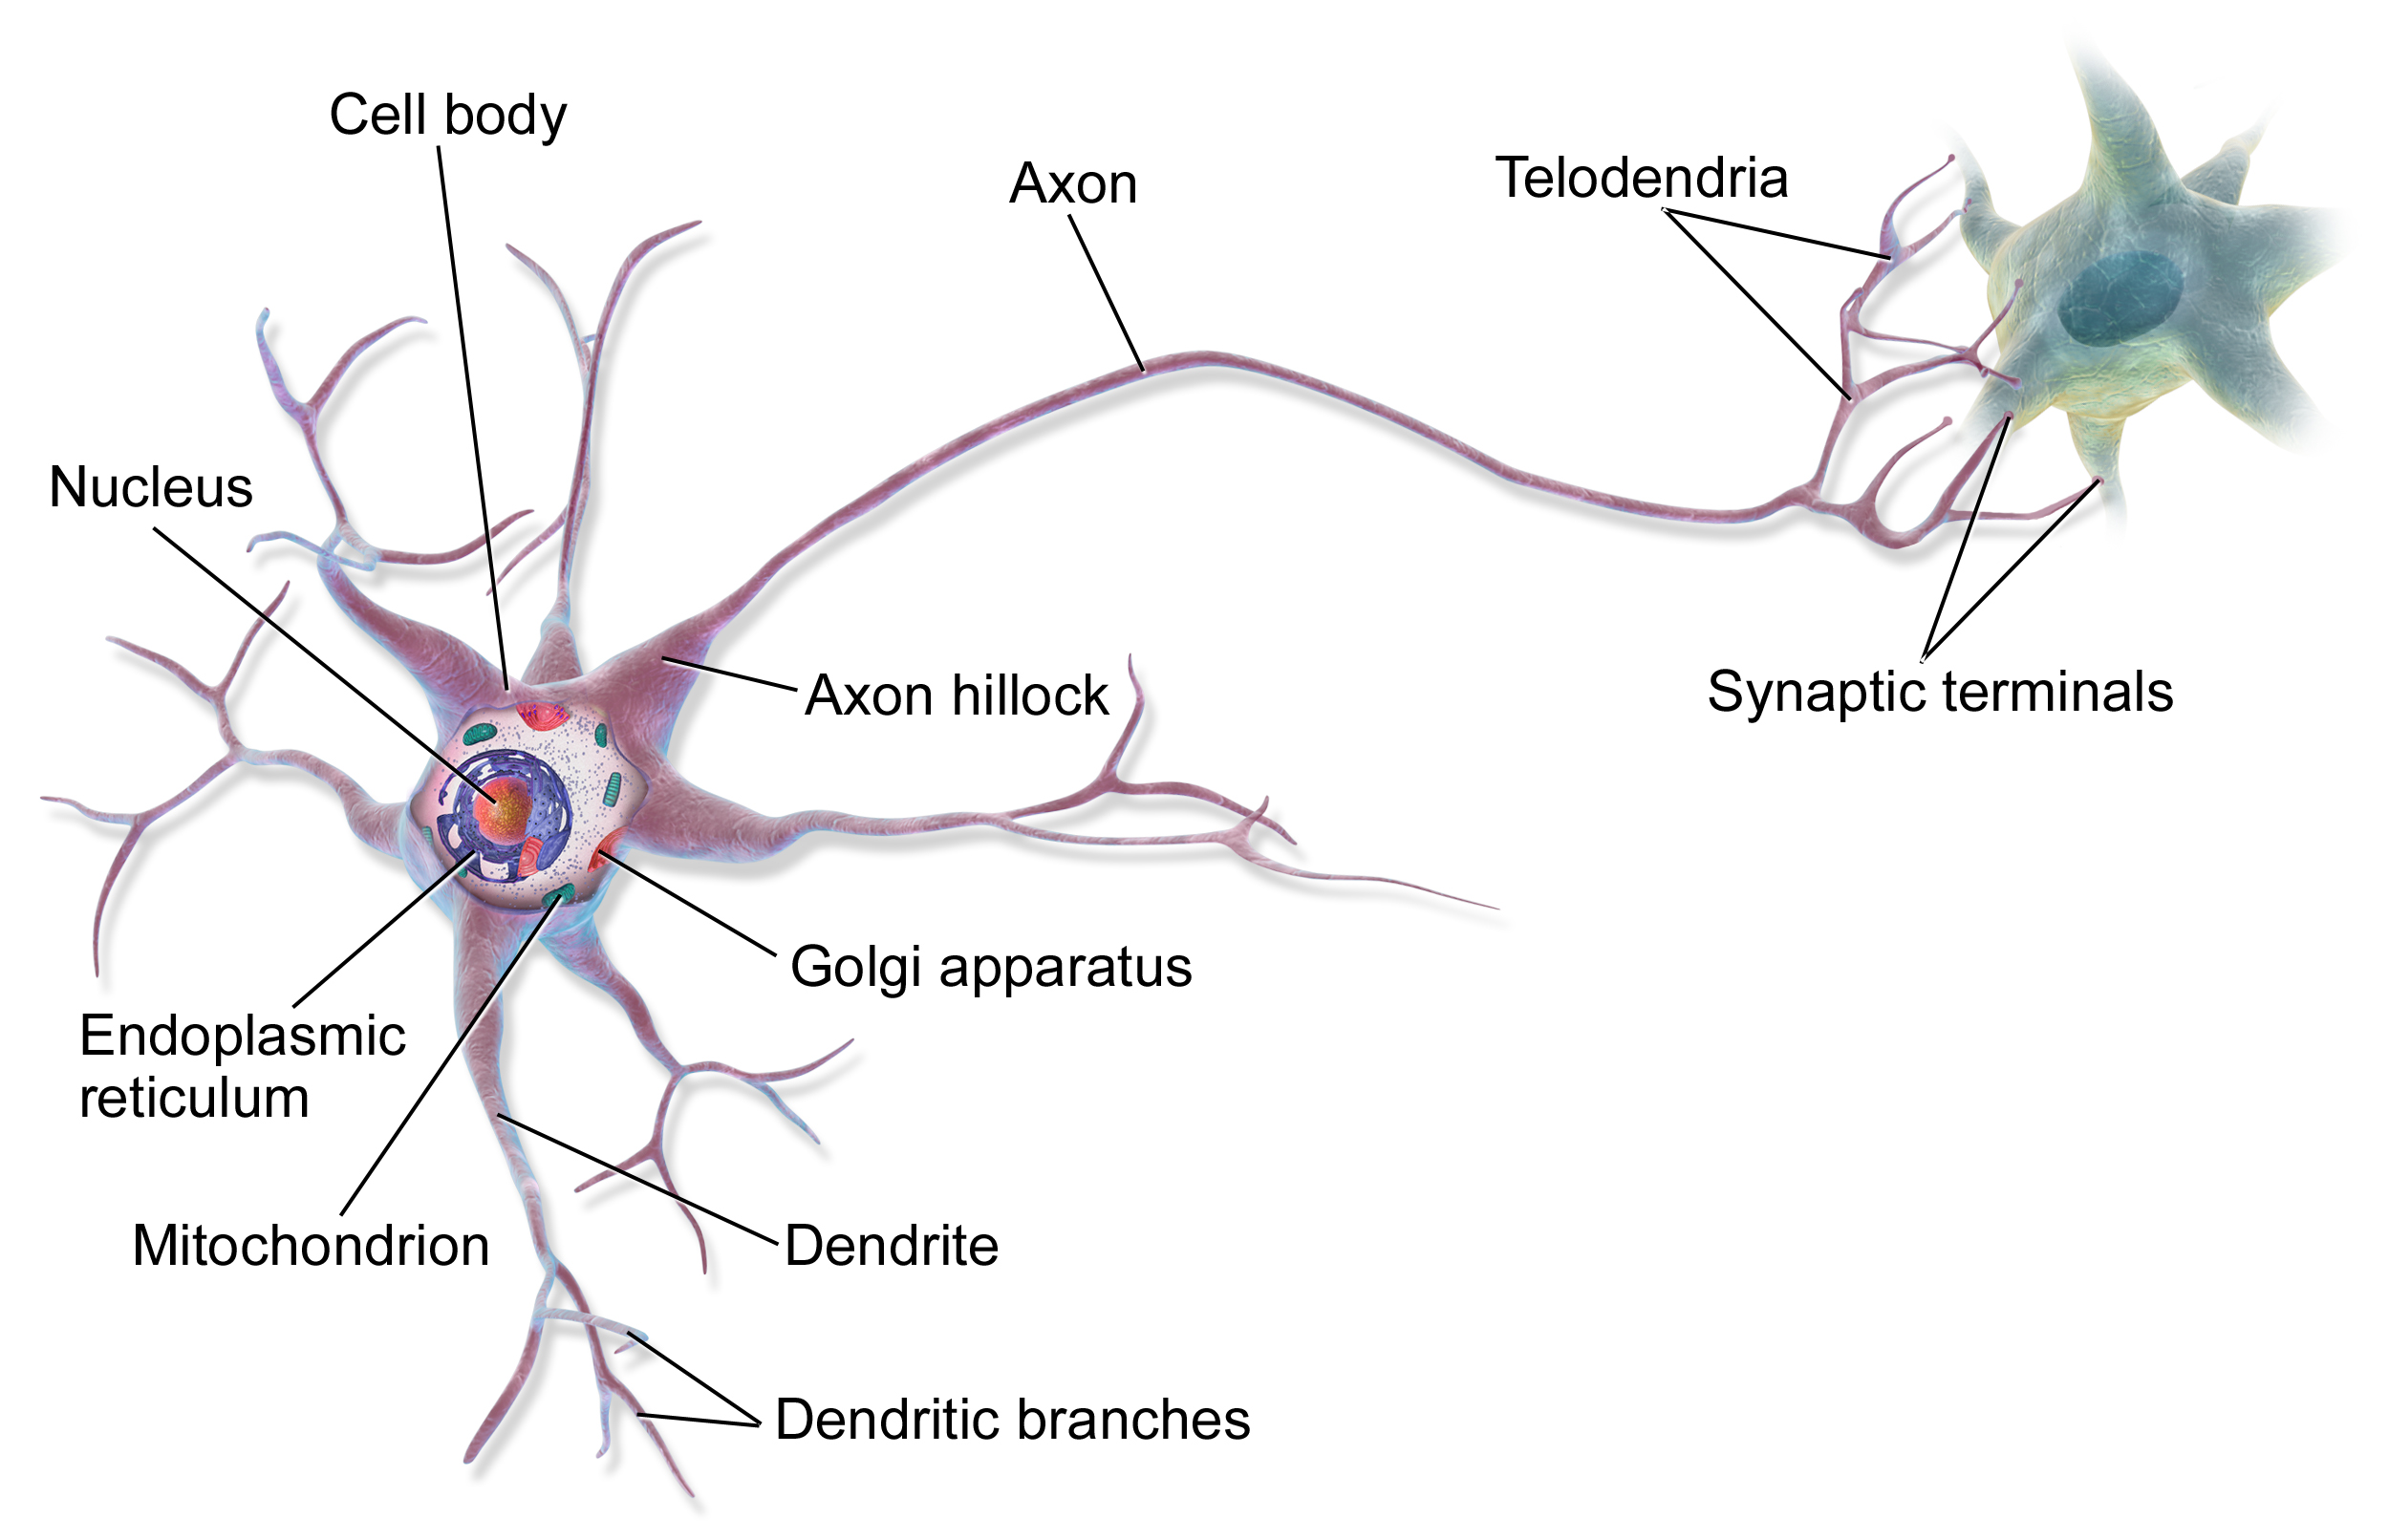
\includegraphics[scale=0.10]{Figures/Blausen_0657_MultipolarNeuron}%
		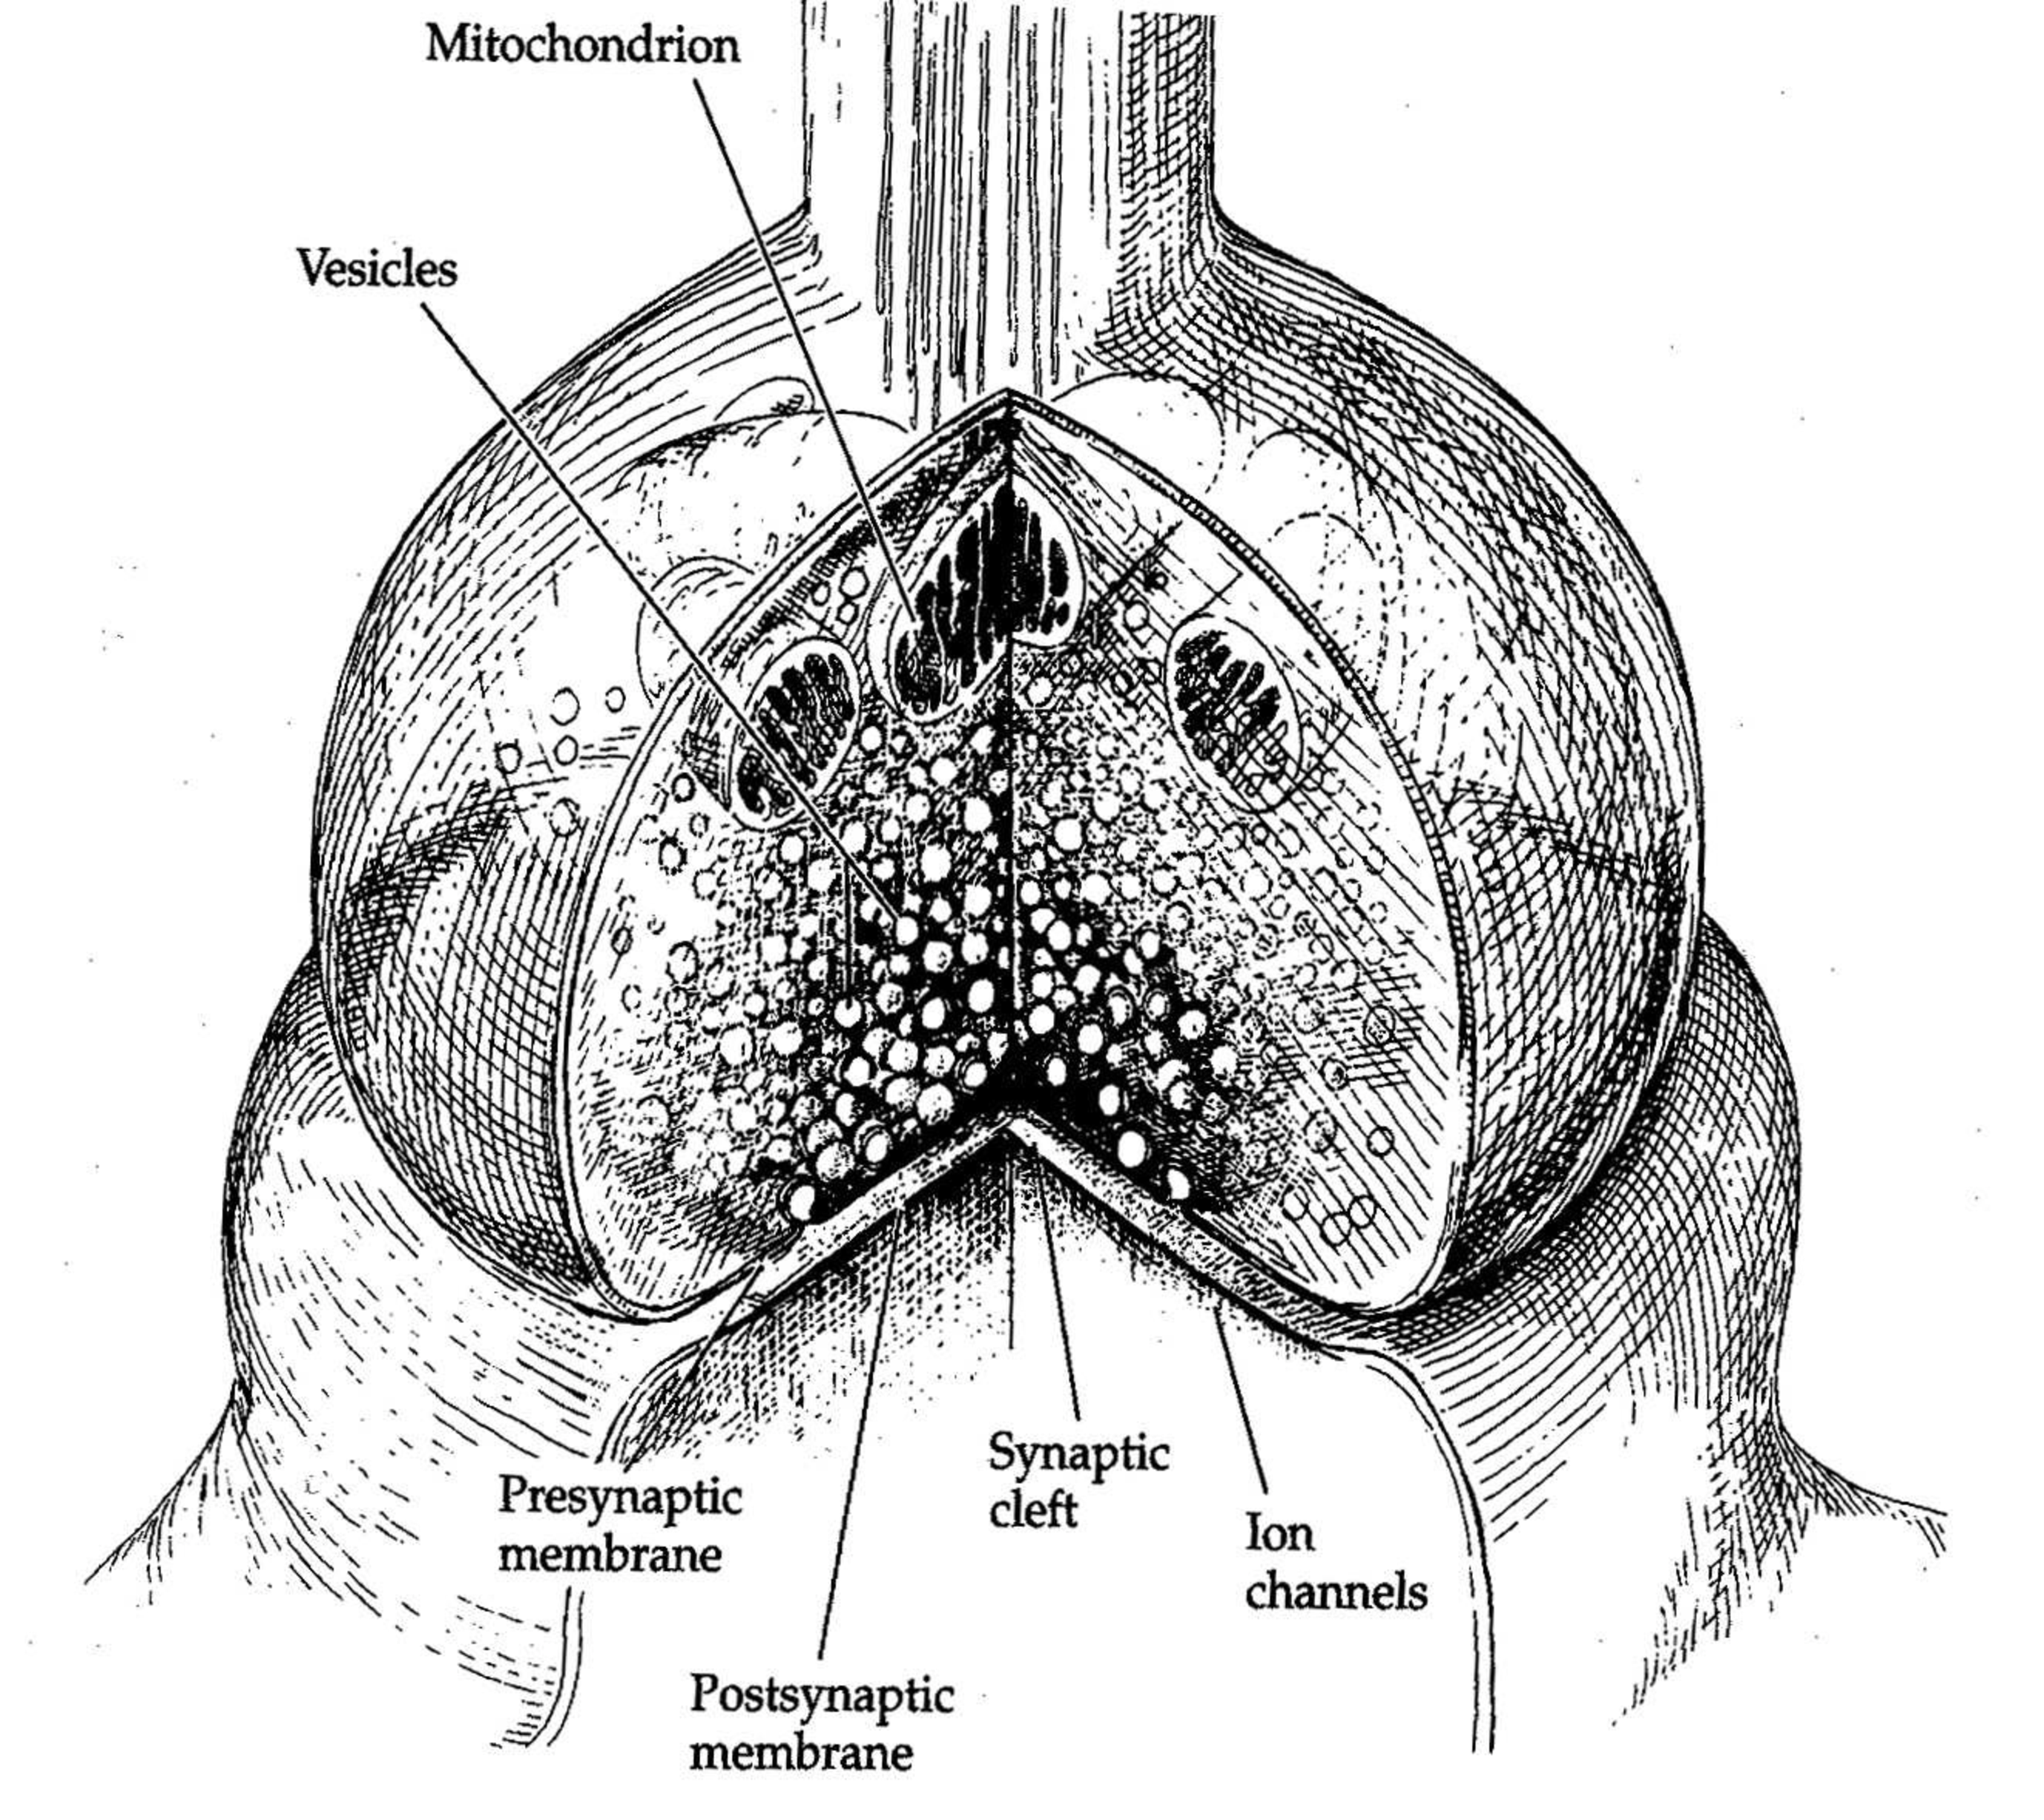
\includegraphics[scale=0.14]{Figures/synapse_drawing}
		\caption{Schematic overview of a neuron. The neurotransmitters are released by the axons of one neuron onto the dendrites of the other.\\ \scriptsize  Left: \url{https://upload.wikimedia.org/wikipedia/commons/1/10/Blausen_0657_MultipolarNeuron.png} \\
		Right: Thompson: ''The Brain'', Worth Publ., 2000}
		\label{fig: drawing neuron and synapse}
	\end{figure}
	
	In this project, I investigate properties of the diffusion process that takes place between the neurons and I solve the congruous 1+1D diffusion equation with a total of five different numerical methods: the backward and forward Euler schemes, the Crank-Nicolson scheme, and Monte Carlo random walk methods using a constant and a distributed step length using a Gaussian distribution.

\section{Theory/Methods}
	The process in question is initiated by an action potential reaching the axon terminal which causes the vesicles inside the axon terminal to join with the pre-synaptic membrane which in turn causes the release of the neurotransmitters into the synaptic cleft. On the other side of the synaptic cleft sits the dendrite, or post-synaptic terminal, which receives the neurotransmitters. Fig.~\ref{fig: synaptic cleft schematic} shows the situation.
	\begin{figure}
		\centering
		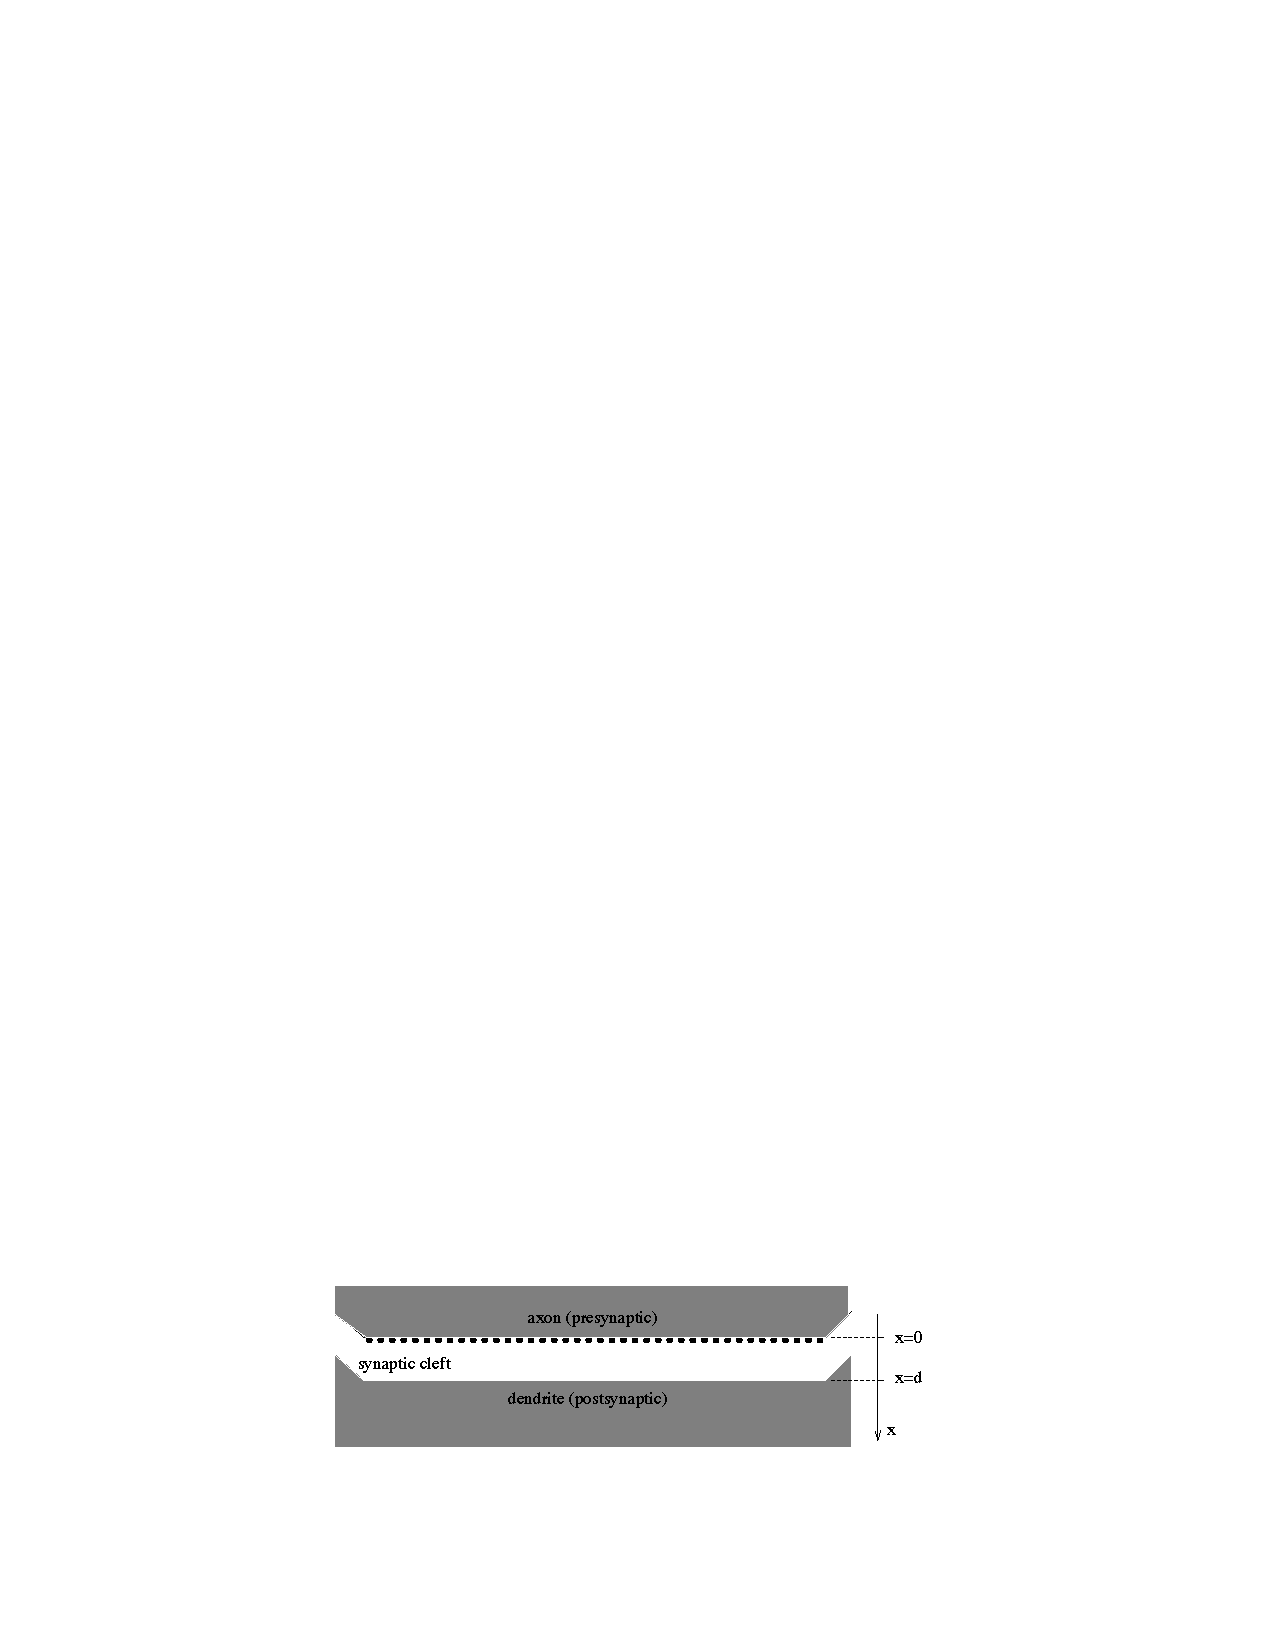
\includegraphics[scale=1]{Figures/synaptic_cleft.pdf}
		\caption{Schematic drawing of the 1D synaptic cleft. The black dots represents a neurotransmitter. The figure shows no neurotransmitters in the synaptic cleft and represents thus the situation immediately after the release of neurotransmitters.}
		\label{fig: synaptic cleft schematic}
	\end{figure}
	
	The diffusion process is governed by the diffusion equation which in three dimension reads
	\begin{align}
		\frac{\partial u}{\partial t} = D\nabla^2u \label{eq: diffusion 1+3D}
	\end{align}
	where $D$ is the diffusion constant and $u$ is the concentration of the neurotransmitter. Eq.~\eqref{eq: diffusion 1+3D} is known as Fick's law after Adolf Eugen Fick who first derived it in 1855. 
	
	In the following, we are assuming that the pre- and post-synaptic surfaces are flat and large in comparison to the width of the synaptic cleft, and that this width is constant across the whole connection. We are also assuming that the neurotransmitters are released equally across the pre-synaptic terminal, that the concentration here is constant and that any neurotransmitters that reach the post-synaptic terminal are immediately  absorbed, leaving the concentration at this point equal to 0.
	
	We can then reduce eq.~\eqref{eq: diffusion 1+3D} to the 1+1D case
	\begin{align}
		\frac{\partial u}{\partial t} = D\frac{\partial^2 u}{\partial x^2} \label{eq: diffusion 1+1D}
	\end{align}
	With boundary conditions
	\begin{align*}
		u(x=0, t>0) = u_0, \qquad u(x=d, \mathrm{all}~t) = 0, \qquad u(0 < x < d, t < 0) = 0
	\end{align*}
	and the initial condition reads
	$$
		u(0 < x < d, 0) = 0
	$$
	
	Since we are, in this project, only interested in the stability of the methods, I will in the following normalize $u_0 = 1$, $D = 1$ and $d = 1$. 
	
	\subsection{Steady state and Analytical solution}
		The above described problem is not trivial to solve either numerically or analytically. A much simpler differential equation is one with boundary conditions 0. I will therefore introduce the \textit{steady state} solution $u_s$ with the property
		\begin{align*}
			\frac{\partial u_s}{\partial t} = 0
		\end{align*}
		with the general solution
		\begin{align*}
			u_s(x) = Ax+b
		\end{align*}
		which, by definition, must have the same boundary conditions as $u$ and so
		\begin{align*}
			u_s(x) = 1-x
		\end{align*}
		This solution is used to define the ''excess'' function for $u$:
		\begin{align*}
			v(x, t) = u(x, t) - u_s(x)
		\end{align*}
		which also satisfies eq.~\eqref{eq: diffusion 1+1D} with boundary and initial conditions 
		\begin{align*}
			v(x, 0) &= u(x, 0) - u_s(x) = 0 - u_s(x) = -u_s(x) = u_0(x)\\
			v(0, t) &= u(0, t) - u_s(0) = 0 \\
			v(1, t) &= u(1, t) - u_s(1) = 0
		\end{align*}
		So we are left solving
		\begin{align}
			\frac{\partial v}{\partial t} = \frac{\partial ^2 v}{\partial x^2} \label{eq: diffusion eq. excess}
		\end{align}
		with the above boundary and initial conditions.
		
		Assuming separation of variables. The excess concentration can then be written in terms of the functions $F(x)$ and $G(t)$ in the following way
		\begin{align*}
			v(x, t) = F(x)G(t)
		\end{align*}
		Inserted in eq.~\eqref{eq: diffusion eq. excess} we get
		\begin{align*}
			F(x)G'(t) &= F''(x)G(t) \\
			\Rightarrow \frac{F''(x)}{F(x)} &= \frac{G'(t)}{G(t)} = -\lambda^2			
		\end{align*}
		where $\lambda$ is a constant. The functions $F(x)$ and $G(t)$ can then be written as
		\begin{align*}
			F(x) &= A\sin(\lambda x) + B\cos(\lambda x) \\
			G(t) &= Ce^{-\lambda^2 t} \\
			\Rightarrow v(x, t) &= \left(A\sin(\lambda x) + B\cos(\lambda x)\right)\cdot Ce^{-\lambda^2 t}
		\end{align*}
		Inserting the boundary condition $v(0, t) = 0$:
		\begin{align*}
			v(0, t) = BCe^{-\lambda^2 t} = 0 \Rightarrow B = 0
		\end{align*}
		since $C=0$ leads to an unphysical solution. The other boundary condition leads to
		\begin{align*}
			&v(1, t) = A\sin(\lambda)\cdot Ce^{-\lambda^2 t} = 0 \\
			\Rightarrow& A\sin(\lambda) = 0 \\
			\Rightarrow& \lambda = n\pi \\
			\Rightarrow& v(x, t) = A_n\sin(n\pi x) e^{-n^2\pi^2t}
		\end{align*}
		or rather, the solution is the linear combination of all possible values of $n$:
		\begin{align}
			v(x, t) = \sum_{n=1}^\infty A_n\sin(n\pi x) e^{-n^2\pi^2 t}
		\end{align}
		where we recognize $A_n$ to be the Fourier coefficient of $v(x, t)$ and can be evaluated in the limit $t=0$.
		We then get
		\begin{align*}
			v(x, 0) = u_0(x) &= \sum_{n=1}^\infty A_n\sin(n\pi x) \\
			\Rightarrow A_n &= 2\int_0^1 u_0\sin(n\pi x) dx
		\end{align*}	
		where I used the property of the Fourier coefficient. We have that $u_0(x) = x-1$. Integration by parts yields
		\begin{align*}
			A_n &= \left.\left(-(x-1)\frac{1}{n\pi}\cos(n\pi x)\right)\right|^1_0 + \frac{1}{n\pi}\int_0^1\cos(n\pi x) dx = \frac{1}{n\pi}
		\end{align*}
		
		And so the solution of the excess-function is
		\begin{align*}
			v(x, t) &= \sum_{n=1}^\infty \frac{1}{n\pi} \sin(n\pi x) e^{-n^2\pi^2t} \\
			\Rightarrow u(x, t) &=  x - 1 + \sum_{n=1}^\infty \frac{1}{n\pi} \sin(n\pi x) e^{-n^2\pi^2t}
		\end{align*}
		
		Below, I will solve $v(x, t)$ as this is much simpler due to the boundary conditions. The linear transformation $v\rightarrow u$ brings no further difficulty to the problem.
		
	\subsection{Forward Euler Scheme}
		In the following, I will use rewrite eq.~\eqref{eq: diffusion 1+1D} as
		\begin{align*}
			\frac{\partial v}{\partial t} = \frac{\partial^2v}{\partial x^2} \Rightarrow v_t = v_{xx}
		\end{align*}
		By a standard Taylor expansion with respect to time of $v(v, t)$ around $t+\Delta t$ results in
		\begin{align*}
			v(x, t+\Delta t) &= v(x, t) + \frac{\partial v(x, t)}{\partial t}\Delta t + \mathcal{O}(\Delta t) \\
			&= v(x, t) + v_t(x, t)\Delta t
		\end{align*}
		or, equivalently
		\begin{align*}
			v_t(x_i, t_j) \approx \frac{v(x_i, t_j + \Delta t) - v(x_i, t_j)}{\Delta t}
		\end{align*}
		Doing the same thing with respect to $x$ to the second order yields
		\begin{align*}
			v_{xx}(x_i, t_i) \approx \frac{v(x_i + \Delta x, t_j) - 2v(x_i, t_j) + v(x_i - \Delta x, t_j)}{\Delta x^2}.
		\end{align*}
		with truncating errors $\mathcal{O}(\Delta t)$ and $\mathcal{O}(\Delta x^2)$ respectively.
		
		This method is explicitly defined by the first point, meaning the first point uniquely defines the following terms. It evolves \textit{forward} and is therefore called the explicit scheme, or the forward Euler method. 
		
		Eq.~\eqref{eq: diffusion 1+1D} then reads in the discretized form
		\begin{align*}
			\frac{v(x_i, t_{j+1}) - v(x_i, t_j)}{\Delta t} &= \frac{v(x_{i+1}, t_j) - 2v(x_i, t_j) + v(x_{i-1}, t_j)}{\Delta x^2} \\
			&\Updownarrow \\
			\frac{v_{i, j+1} - v_{i, j}}{\Delta t} &= \frac{v_{i+1, j} - 2v_{i, j} + v_{i-1, j}}{\Delta x^2}
		\end{align*}
		which leads to
		\begin{align}
			\Rightarrow v_{i, j+1} &= \alpha v_{i-1,j} + (1-2\alpha)v_{i,j} + \alpha v_{i+1,j}\label{eq: forward euler}
		\end{align}
		where $\alpha = \Delta t/\Delta x^2$. So, we see that the next point in time is explicitly defined by the previous at three points in space. This in mind, one could device the following algorithm in C++:
		\begin{lstlisting}
// Assuming that u and unew is initialized 
// and u initially contains the initial condition
t_stop = 0.1; // How long you want the simulation to go
dt     = ;// Choose some time-step
dx     = ;//Choose some x-step
alpha = dt/(dx*dx);
for (int j = 0; T <= t_stop; j++) {
     for (int i = 1; i < N_x - 1; i++) {
          unew[i] = alpha*(u[i-1] + u[i+1]) + (1 - 2*alpha)*u[i];
     }
     u = unew;
     T += dt;
}
		\end{lstlisting}
		
		\subsubsection{Matrix-Vector and Stability}
			Another way of solving eq.~\eqref{eq: forward euler} is by the matrix-vector equation
			\begin{align*}
				\mathbf{v}_{j+1} = \mathbf{A}\mathbf{v}_j = \mathbf{A}^{j+1}\mathbf{v}_0
			\end{align*}
			where the vector $\mathbf{v}_j$ contains all the $v_{i,j}$'s at time step $j$ and
			\begin{align*}
				A =	
				\begin{bmatrix}
					1-2\alpha & \alpha & 0 & 0 & \cdots & \cdots \\
					\alpha		& 1-2\alpha & \alpha & 0 & \cdots & \cdots \\
					0 & \alpha & 1-2\alpha & \alpha & 0 & \cdots \\
					\cdots & \cdots & \cdots & \cdots & \cdots & \cdots \\
					0& 0 & \cdots & \cdots & \alpha & 1-2\alpha
				\end{bmatrix}
			\end{align*}
			is tridiagonal.
			
			As with any exponential function, it is convergent only if the base is less than 1. It can be shown that the tridiagonal matrix above is positive definite, and so the above equation can be converted into an eigenvalue problem. Thus, for convergence, we require the largest eigenvalue of $A$ to be smaller than one, equivalent to the spectral radius
			\begin{align*}
				\rho(\mathbf{A}) = \mathrm{max}\{|\lambda|: \mathrm{det}(\mathbf{A}-\lambda\mathbf{I}) = 0\} < 1
			\end{align*}
			Where $\mathbf{I}$ is the identity matrix.
			
			Let 
			\begin{align*}
				\mathbf{A} = \mathbf{I} - \alpha\mathbf{B}
			\end{align*}
			where
			\begin{align*}
				\mathbf{B} = 
				\begin{bmatrix}
					2 & -1 & 0 & 0 & \cdots \\
					-1 & 2 & -1 & 0 & \cdots \\
					\cdots & \cdots & \cdots & \cdots & -1 \\
					 0 & 0 & \cdots & -1 & 2
				\end{bmatrix}
			\end{align*}
			which is a tridiagonal Toeplitz matrix with known eigenvalues\cite{pasquini2006tridiagonal}. A brief version of the proof is included.
			
		The eigenvalues of $\mathbf{A}$ are  $\lambda_i = 1 - \alpha \mu_i$ where $\mu_i$ is the eigenvalues of $\mathbf{B}$. The elements of $\mathbf{B}$ can be written as
		\begin{align*}
			b_{ij} = 2\delta_{ij} -\delta_{i+1j} - \delta_{i-1j}
		\end{align*}
		where $\delta$ is the Kronecker delta function. To find $\mu_i$ we then have
		\begin{align*}
			(\mathbf{B}\mathbf{x})_i =\sum_{j=1}^n(2\delta_{ij} -\delta_{i+1j} - \delta_{i-1j})x_j = 2x_i-x_{i+1} - x_{i-1}= \mu_ix_i
		\end{align*}
		Assuming that $\mathbf{x}$ can be written in the basis $(\sin(\theta), \sin(2\theta),..., \sin(n\theta))$ with $\theta = \theta(n)$, we end up with
		\begin{align*}
			\mu_i\sin(i\theta) &= 2\sin(i\theta) - \sin((i+1)\theta) - \sin((i-1)\theta) \\
			&= 2(1-\cos(\theta))\sin(i\theta) \\
			\Rightarrow \mu_i &= 2(1-\cos(\theta)) \\
			\Rightarrow \lambda_i &= 1-2\alpha(1-\cos(\theta))
		\end{align*}
		Thus the requirement reads
		\begin{align*}
			-1 < 1 - 2\alpha(1-\cos(\theta)) < 1
		\end{align*}
		or
		\begin{align*}
			\alpha < (1 - \cos(\theta))^{-1} \Rightarrow \alpha \leq \frac{1}{2}
		\end{align*}
		which in turn gives us the stability condition for the explicit scheme:
		\begin{align}
			\frac{\Delta t}{\Delta x^2} \leq \frac{1}{2} \label{eq: forward euler stability}
		\end{align}
	
	\subsection{Backward Euler Scheme}
		Instead of performing the Taylor expansion around $t+\Delta t$ as in the explicit scheme, another possibility is
		\begin{align*}
			v(x, t-\Delta t) &= v(x, t) - \frac{\partial v(x, t)}{\partial y} \Delta t + \mathcal{O}(\Delta t) \\
			&= v(x, t) - v_t(x, t)\Delta t + \mathcal{O}(\Delta t)
		\end{align*}
		or in the discretized form
		\begin{align*}
			v_t \approx \frac{v_{i,j} - v_{i,j-1}}{\Delta t}
		\end{align*}
		Leaving the $x$-derivative unchanged, we get
		\begin{align}
			\frac{v_{i,j} - v_{i, j-1}}{\Delta t} &= \frac{v_{i+1,j} - 2v_{i,j} + v_{i-1,j}}{\Delta x^2} \nonumber \\
			v_{i,j-1} &= -\alpha v_{i-1,j} +(1-2\alpha)v_{i,j} -\alpha v_{i+1,j} \label{eq: backward euler}
		\end{align}
		leaving us with what is known as the backward Euler, or the implicit scheme.
		
		\subsubsection{Matrix-Vector and Stability}
			Again, we can rewrite eq.~\eqref{eq: backward euler} as a matrix-vector equation
			\begin{align*}
				\mathbf{v}_{j-1} &= \mathbf{A}\mathbf{v}_j \\
				\mathrm{or} \qquad \mathbf{v}_j &= \mathbf{A}^{-1}\mathbf{v}_{j-1}
			\end{align*}
			where $\mathbf{A}$ is as previously defined. By the same token as in the previous section, it can be shown that the spectral radius $\rho(\mathbf{A}^{-1}) < 1$ for all choices of $\Delta t$ and $\Delta x$. 
			
			In project 1 of this course, I devised a method of solving such sets of tridiagonal matrix equations\cite{project1}, involving the LU-decomposition of $\mathbf{A}$. 
			
			The following code reuses the code from project 1 to solve the equation. The code should be self-explanatory.
			\begin{lstlisting}
for (int i = 0; T <= t_stop; i++) {
   for (int j = 0; j < N_x; j++) {
       a[j] = -alpha;
       b[j] = 1 + 2*alpha;
       c[j] = -alpha;
   }
   forward_substitution(a, b, c, u, N_x);
   backward_substitution(b, c, u, unew, N_x);
   // the boundary conditions may be changed in the tridiag solver. 
   // Need to change them back
   unew[0] = u[0];
   unew[N_x-1] = u[N_x-1];

   // update the known vector
   u = unew;
   T += dt;
}
			\end{lstlisting}
			
			
			\subsection{Crank-Nicolson Scheme}
				While both the forward and backward Euler schemes have a truncation error of $\Delta t$ and $\Delta x^2$ respectively, we can make a method which has a truncation error of $\Delta t^2$ and $\Delta x^2$.
				
				The resulting method is named after its developers John Crank and Phyllis Nicolson - the Crank-Nicolson cheme. The Crank-Nicolson scheme uses a time-centered approximation for the derivatives $v_{t}$ and $v_{xx}$ and similar to above we find express the next timestep $v(x, t+\Delta t)$ and spatial-step $v(x+\Delta x, t)$ as Taylor expansions, but around $t'=t+\Delta t/2$.
				
				This is to say, the time-derivative is the average of the derivatives at time-step $j$ and $j+1$, i.e. time-centred between two time-points. Taking the backward Euler scheme at $j+1$ yields
				\begin{align*}
					v_t (BE) = \frac{v_{i,j+1} - v_{i,j}}{\Delta t}
				\end{align*}
				the same as for backward Euler. The corresponding spatial derivative at $j+1$ is
				\begin{align*}
					v_{xx} (BE) = \frac{v_{i+1,j+1} - 2v_{i,j+1}+v_{i-1,j+1}}{\Delta x^2}
				\end{align*}
				The average of the BE-method at $j+1$ and FE at $j$, gives us finally the time-centred Crank-Nicolson scheme:
				\begin{align}
					\frac{1}{2}( v_t (\mathrm{BE~at~}j+1) + v_t(\mathrm{FE~at~}j) =\frac{1}{2}( v_{xx}(\mathrm{BE~at~}j+1) + v_{xx}(\mathrm{FE~at~}j)) \nonumber \\
					\Rightarrow\frac{v_{i,j+1}-v_{i,j}}{\Delta t} = \frac{1}{2}\left[\frac{v_{i+1,j+1} - 2v_{i,j+1} + v_{i-1,j+1}}{\Delta x^2} + \frac{v_{i+1,j} - 2v_{i,j} + v_{i-1,j}}{\Delta x^2}\right]
				\end{align}
				Since we are taking the average, the truncation errors become $\Delta t^2$ and $\Delta x^2$.
				
		Using again our previous definition of $\alpha = \Delta t / \Delta x^2$, we obtain
		\begin{align}
			(2-2\alpha)v_{i,j} + \alpha v_{i-1,j} + \alpha v_{i+1,j} &= (2\alpha + 2)v_{i,j+1} - \alpha v_{i+1,j+1} - \alpha v_{i-1,j+1}
		\end{align}
	
		\subsubsection{Matrix-Vector and Stability}
			One can quite easily see that the above difference equation can be written as a matrix-vector equation as
			\begin{align}
				(2\mathbf{I} + \alpha \mathbf{B})\mathbf{v}_{j+1} = (2\mathbf{I} - \alpha\mathbf{B})\mathbf{v}_j \label{eq: CN scheme matrix vector}
			\end{align}
			where $\mathbf{B}$ is like previously defined. The equation can be rewritten as
			\begin{align*}
				\mathbf{v}_{i+1} = (2\mathbf{I} + \alpha \mathbf{B})^{-1}(2\mathbf{I} - \alpha \mathbf{B})\mathbf{v}_j
			\end{align*}
			where the spectral radius
			\begin{align*}
				\rho((2\mathbf{I} + \alpha \mathbf{B})^{-1}(2\mathbf{I} - \alpha \mathbf{B})) < 1
			\end{align*}
			and thus, is this method stable for all choices of $\Delta t$ and $\Delta x$.
			
			The implementation of the CN scheme is somewhat simple, now that we already have an implementation for the backward and forward schemes. Rewriting eq.~\eqref{eq: CN scheme matrix vector}
			\begin{align*}
				\mathbf{C}\mathbf{v}_j = \mathbf{C}'\mathbf{v}_{j-1}
			\end{align*}
			we see that the right hand side is known. If we label this $\hat{\mathbf{v}}_{j-1}$, we obtain
			\begin{align*}
				\mathbf{C}\mathbf{v}_j = \hat{\mathbf{v}}_{j-1}
			\end{align*}
			which is just the backward Euler scheme. The implementation in C++ could then look similar to the following
			\begin{lstlisting}
// boundary conditions:
unew[0] = u[0]; unew[N_x - 1] = u[N_x - 1];
RHS[0] = u[0]; RHS[N_x - 1] = u[N_x - 1];
double alpha = dt/dx/dx;
double T = 0;
for (int i = 0; T <= t_stop; i++) {
     // calculating RHS
     for (int j = 1; j < N_x - 1; j++) {
          RHS[j] = alpha*(u[j-1] + u[j+1]) + (2 - 2*alpha)*u[j];
     }
        
     // now calculate the tridiagonal linear eq.
     // first, set up the matrix
     for (int j = 0; j < N_x; j++) {
          a[j] = -alpha;
          b[j] = 2 + 2*alpha;
          c[j] = -alpha;
     }
     forward_substitution(a, b, c, RHS, N_x);
     backward_substitution(b, c, RHS, unew, N_x);
     // The boundary conditions are changed by forward/backward substitution. 
     //Need to change them back.
     unew[0] = u[0]; unew[N_x - 1] = u[N_x - 1];
     RHS[0] = u[0]; RHS[N_x - 1] = u[N_x - 1];
     
     unew = u;     
     T += dt;
}
			\end{lstlisting}
			
	
	\subsection{Random walk}
		The final method studied, is the method of random walks. It assumes that every single particle is can be modelled as a random walker with equal probability of walking to the right and to the left in the 1D synaptic cleft. The implementation is really quite simple as long as we remember the physical conditions of the system. Assume we store the position of each random walker/particle in an array of length equal to the number of particles in the system. The physical conditions then require the following.
		
		Firstly, the initial concentration is zero throughout the synaptic cleft and all particles start off at the axon terminal. The first condition is 
		\begin{itemize}
			\item[i)] All particles start off at $x=0$
		\end{itemize}
		The concentration at this point must be conserved, because of the boundary conditions, and so the second and third conditions must be satisfied
		\begin{itemize}
			\item[ii)] If a particle leaves $x=0$, then another particle must take its place, extending the position array by one element.
			\item[iii)] if a particle has left $x=0$ for some time and comes back, it must be immediately taken away to conserve the particle number at $x=0$. The same applies if a particle goes past $x=0$ leaving its position negative.
		\end{itemize}
		The final condition concerns the concentration at $x=1$, the end point
		\begin{itemize}
			\item[iv)] if a particle hits the wall at $x=1$, it is immediately absorbed and removed from the position array, effectively reducing the size by 1.
		\end{itemize}
		
		Because of numerical imprecision, conditions iii) and iv) should, instead of being sharply defined, accept in a small range $\varepsilon < 10^{-4}$ or so.
		
		\subsubsection{Constant Step Length}
			I have argued that the diffusion process can be modelled as a series of random walkers, however the length of each step is not discussed. We can compute the mean displacement and the mean of the square of the displacement using the following
			\begin{align}
				\langle x(t)\rangle &= \int_{-\infty}^\infty xu(x, t) dx \\
				\mathrm{and} \qquad \langle x^2(t) \rangle &= \int_{-\infty}^\infty x^2u(x, t)dx
			\end{align}
			which come to $0$ and $2D\Delta t$ respectively\cite{farnell2005monte}, and so the variance, or root mean square of the displacement is
			\begin{align*}
				l_0 = \sqrt{\langle x^2\rangle - \langle x \rangle} = \sqrt{2D\Delta t} = \sqrt{2\Delta t}
			\end{align*}
			where $D=1$.
		
		\subsubsection{Gaussian Step Length}
			It is, however, reasonable to believe that the step length a real random walker would take is not constant, but falls within a bell curve with standard deviate $l_0$, and so we could use a random number generator to generate Gaussian numbers $\xi$ with standard deviate 1 and mean value 0, to calculate the step length using $$l_0 = \sqrt{2\Delta t}\xi.$$
			
			We must now, however, consider the fact that a particle may initially move to the right, but not beyond $\varepsilon$ below which we should delete it, according to condition iii) above. If this is the case, it should not be removed. If, however, it has had a position $x>\varepsilon$ and moved to a position $x<\varepsilon$, it should be removed. 
			
	
\section{Results and Discussion}
	\subsection{Differential schemes}
		Fig.~\ref{fig: differentials all results} shows the results of four different runs of the program that calculates $u(x, t)$ for $\Delta x= \{1/10, 1/100\}$. All units are relative since they have been normalized so that $d=1$ and $D = 1$. The figure also shows the relative first degree error of the three methods and it is very obvious that all three methods are reasonably accurate with errors in the order of$10^{-4}$ - $10^{-2}$ percent. Table~\ref{table: errors from differential methods} shows the root mean square error of the calculations as calculated by the standard deviate of the difference between the data points in the analytical and numerical methods.
		
		The time-step for the forward Euler scheme is that dictated by the stability condition eq.~\eqref{eq: forward euler stability} and for the other methods it has been chosen very small, $\Delta t = 5\cdot 10^{-9}$ for better performance. 
		
		The table and figure shows clearly the advantage of the more sophisticated methods as the error decreases dramatically, however the forward Euler is much faster than its competitors, using only in the order of $O(6n)$ FLOPS, whereas the other methods uses $O(10n)$ and $O(16n)$ FLOPS per time iteration for the backward Euler and Crank-Nicolson schemes respectively, since the LU-decomposition uses $O(10n)$ FLOPS\cite{project1}. One is also likely to stumble upon overflow when dealing with small step-lengths, as the matrix becomes increasingly large with smaller $\Delta x$.

\begin{table}
\centering
\caption{Root mean square error for the different differential methods for different steps $\Delta x$ and at two time points in the simulation.}
\label{table: errors from differential methods}
\begin{tabular*}{\textwidth}{l@{\extracolsep{\fill}}ccc}
\multicolumn{1}{c}{Method}      & \multicolumn{1}{c}{$\Delta x$ [Rel. units]}   & $\epsilon(T=0.1)$ [\%] & $\epsilon( T=0.3)$ [\%] \\ \hline \hline
\multirow{2}{*}{Forward Euler}  	& 0.1  	& $4.44\cdot 10^{-1}$  & $8.28\cdot 10^{-2}$  \\
                               			 		& 0.01	& $7.11\cdot 10^{-3}$  & $1.22\cdot 10^{-3}$  \\ \hline
\multirow{2}{*}{Backward Euler}	& 0.1  	& $2.03\cdot 10^{-2}$  & $1.69\cdot 10^{-2}$  \\
                                					& 0.01	& $1.88\cdot 10^{-4}$  & $1.68\cdot 10^{-4}$  \\ \hline
\multirow{2}{*}{Crank-Nicolson} & 0.1 	& $2.03\cdot 10^{-2}$  & $1.69\cdot 10^{-2}$  \\
                                					& 0.01	& $1.84\cdot 10^{-4}$  & $1.65\cdot 10^{-4}$  \\ 
\end{tabular*}
\end{table}
		\afterpage{
		\begin{figure}
			\centering
			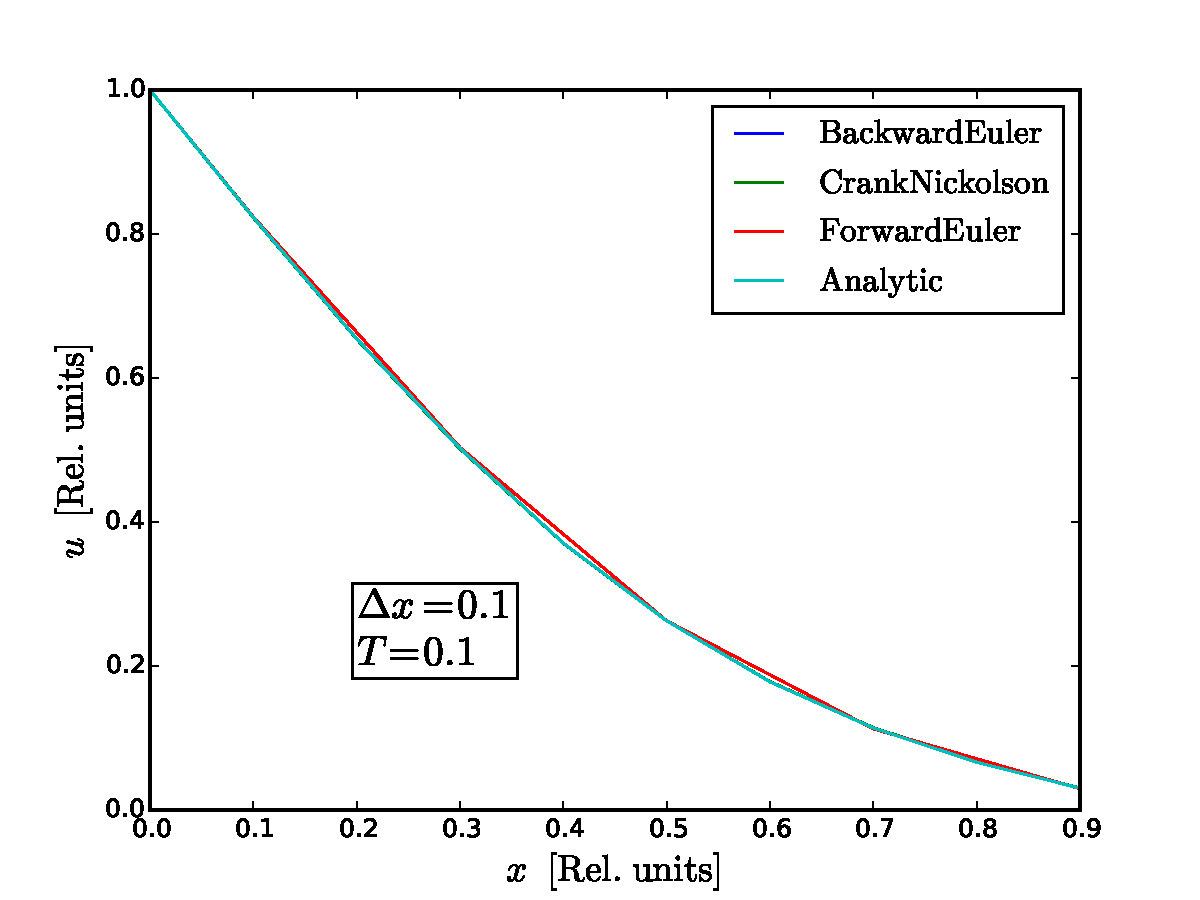
\includegraphics[width=0.49\linewidth, clip=true, trim=0 5 0 29]{Figures/FYS3150_project_5_differential_dx01_curved.pdf}%
			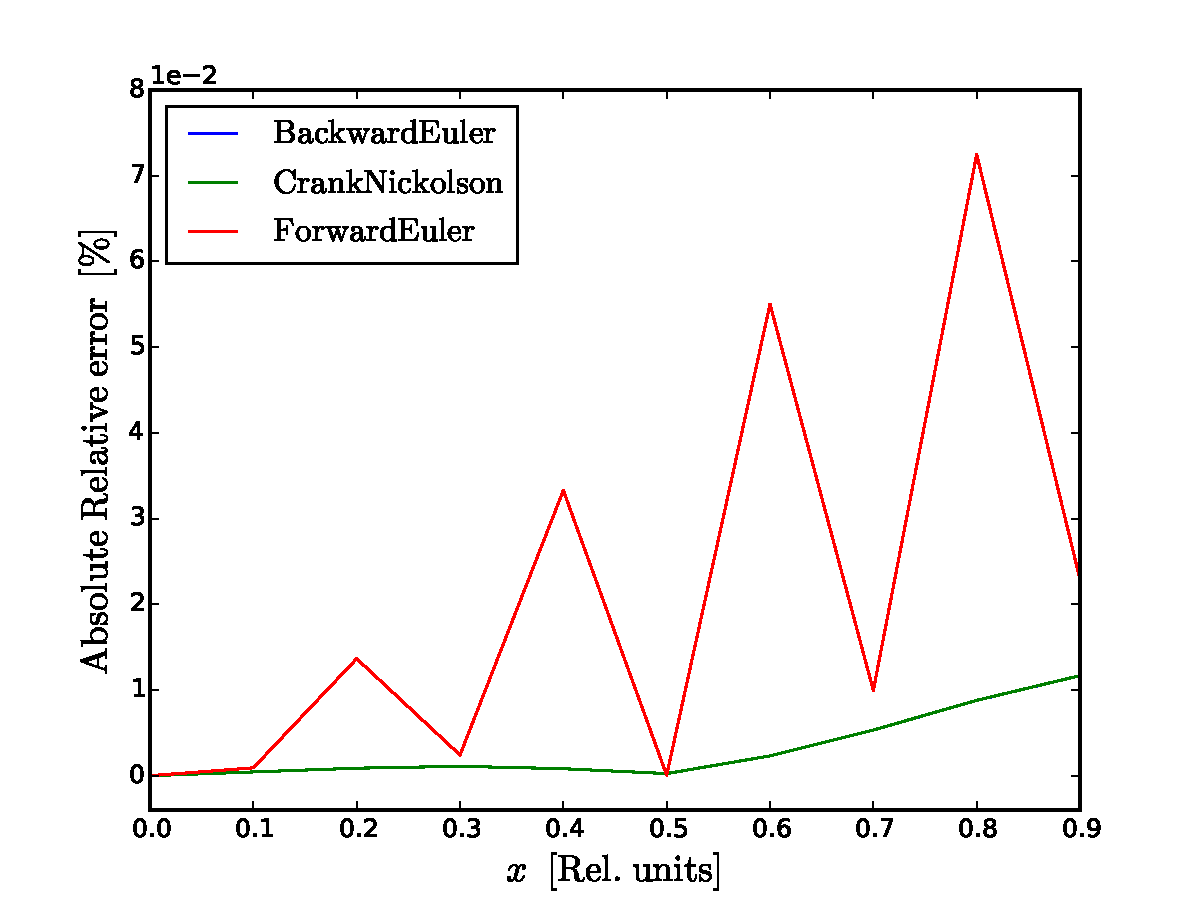
\includegraphics[width=0.49\linewidth, clip=true, trim=0 5 0 29]{Figures/FYS3150_project_5_differential_error_dx01_curved.pdf}

			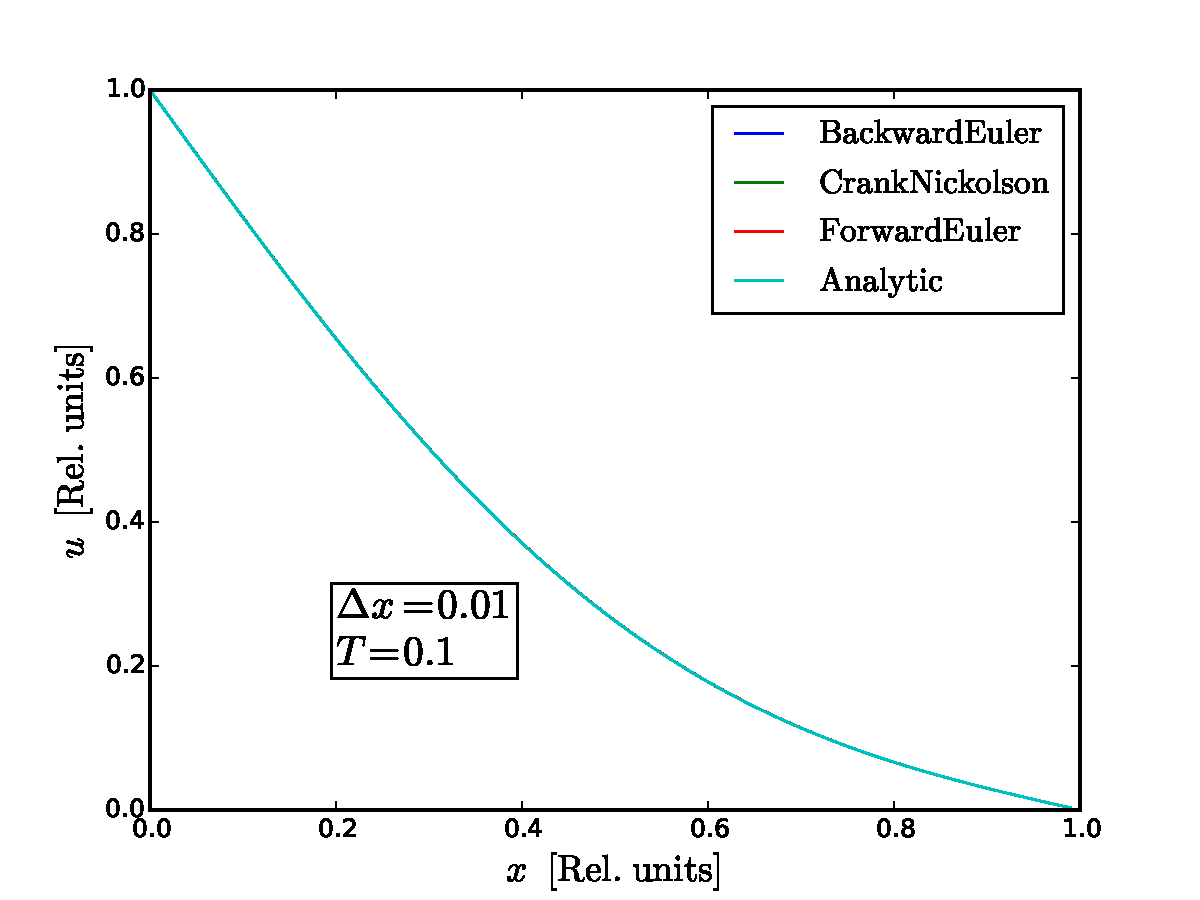
\includegraphics[width=0.49\linewidth, clip=true, trim=0 5 0 29]{Figures/FYS3150_project_5_differential_dx001_curved.pdf}%
			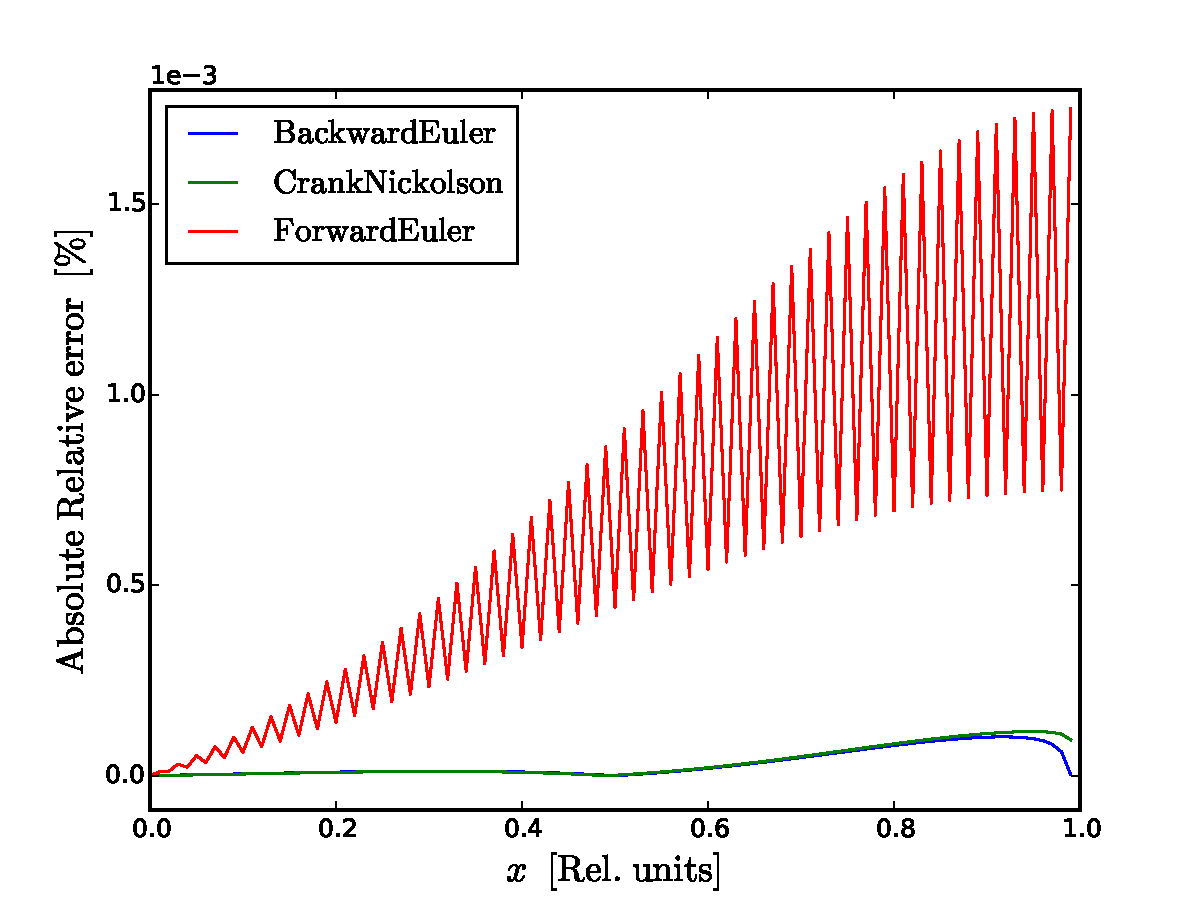
\includegraphics[width=0.49\linewidth, clip=true, trim=0 5 0 29]{Figures/FYS3150_project_5_differential_error_dx001_curved.pdf}

			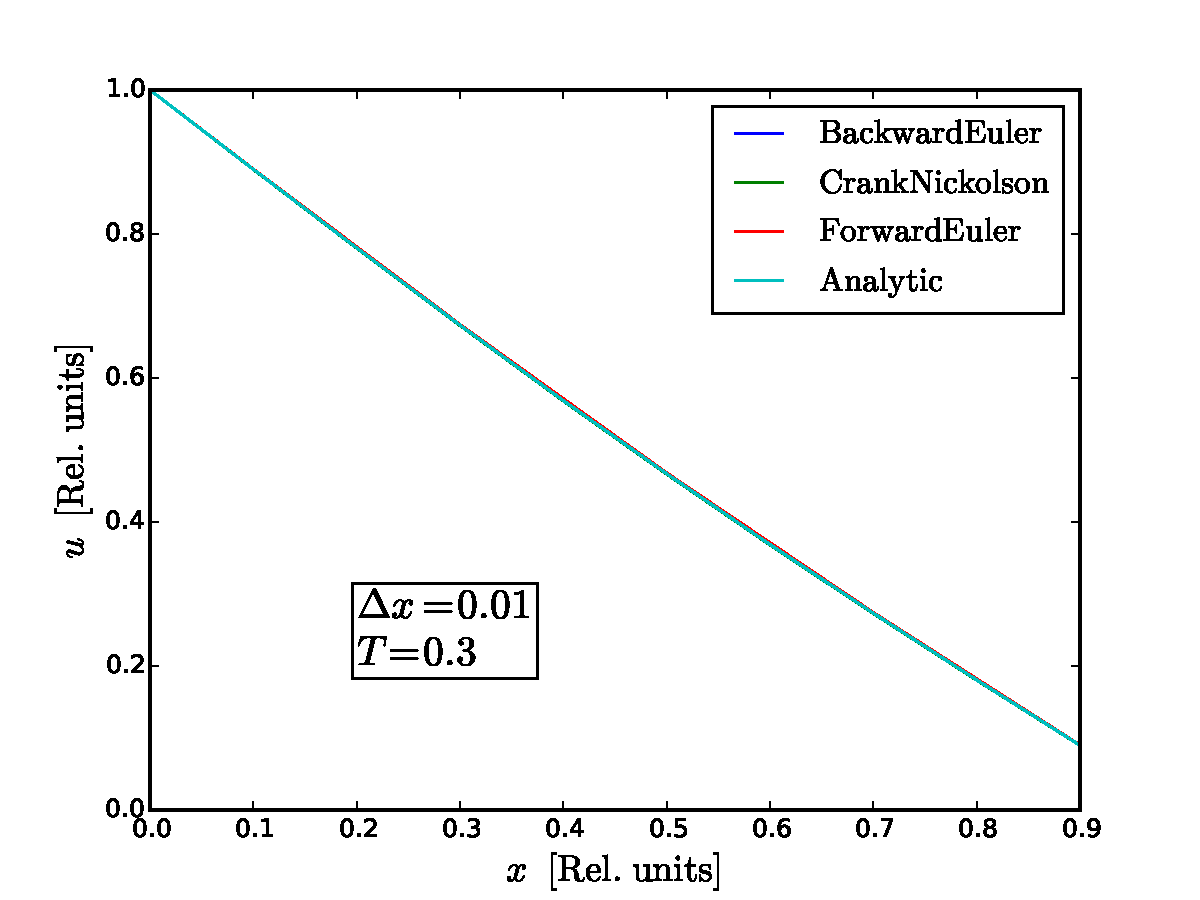
\includegraphics[width=0.49\linewidth, clip=true, trim=0 5 0 29]{Figures/FYS3150_project_5_differential_dx01_linear.pdf}%
			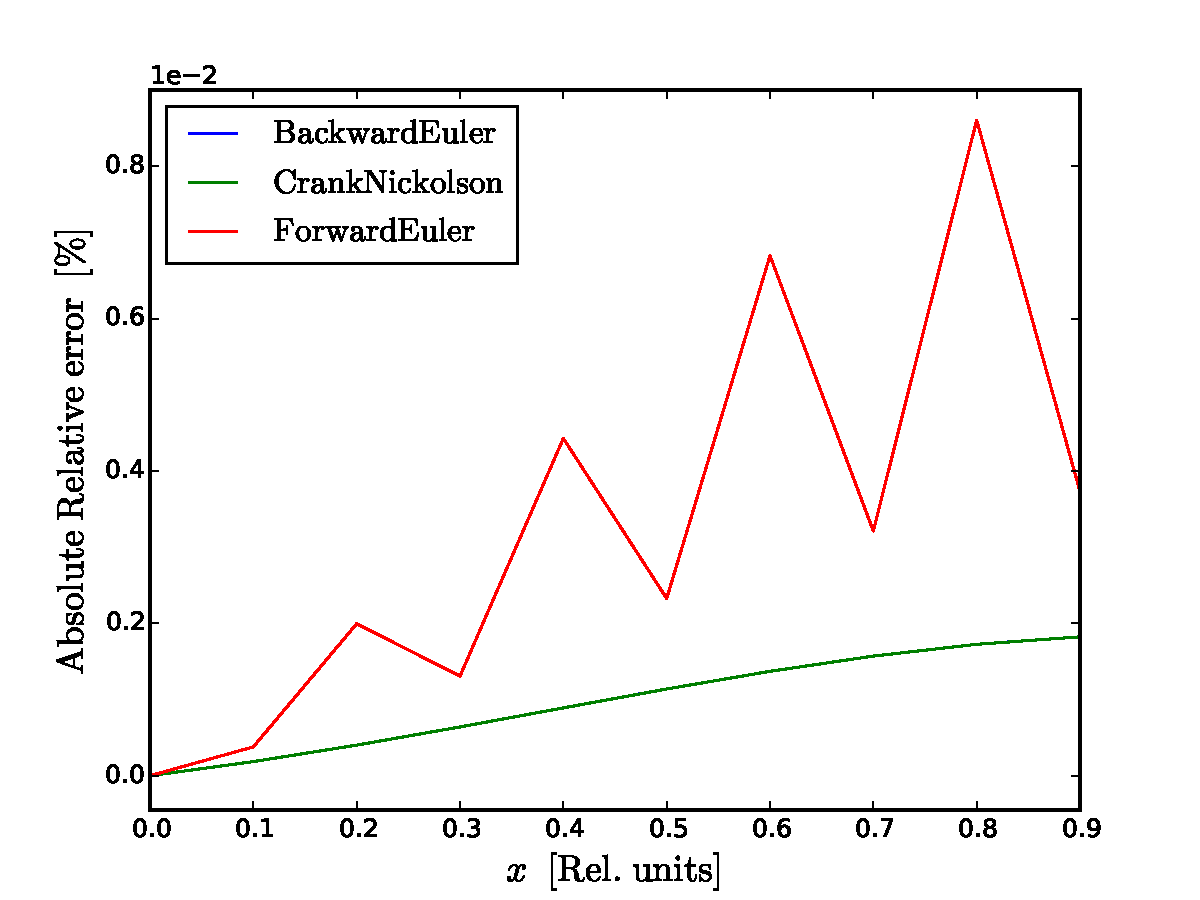
\includegraphics[width=0.49\linewidth, clip=true, trim=0 5 0 29]{Figures/FYS3150_project_5_differential_error_dx01_linear.pdf}

			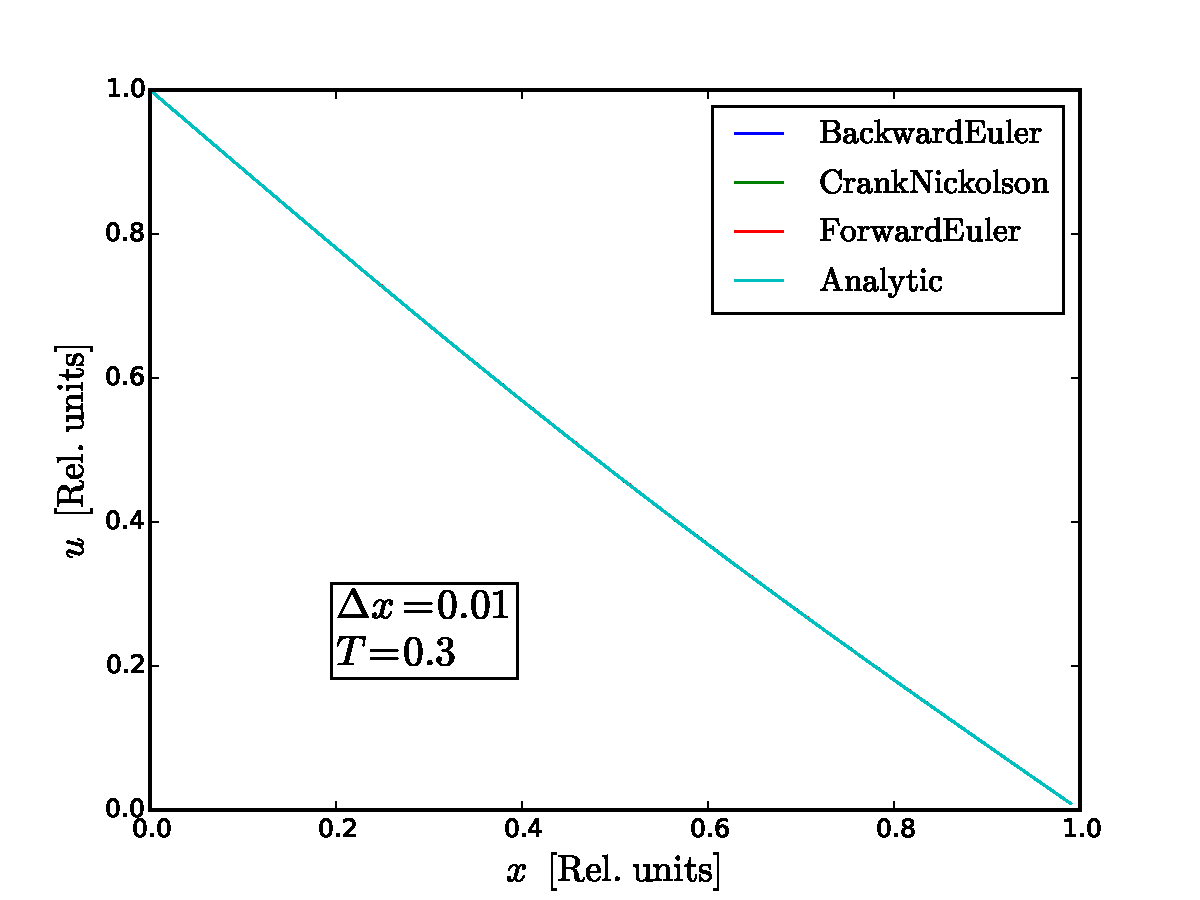
\includegraphics[width=0.49\linewidth, clip=true, trim=0 5 0 29]{Figures/FYS3150_project_5_differential_dx001_linear.pdf}%
			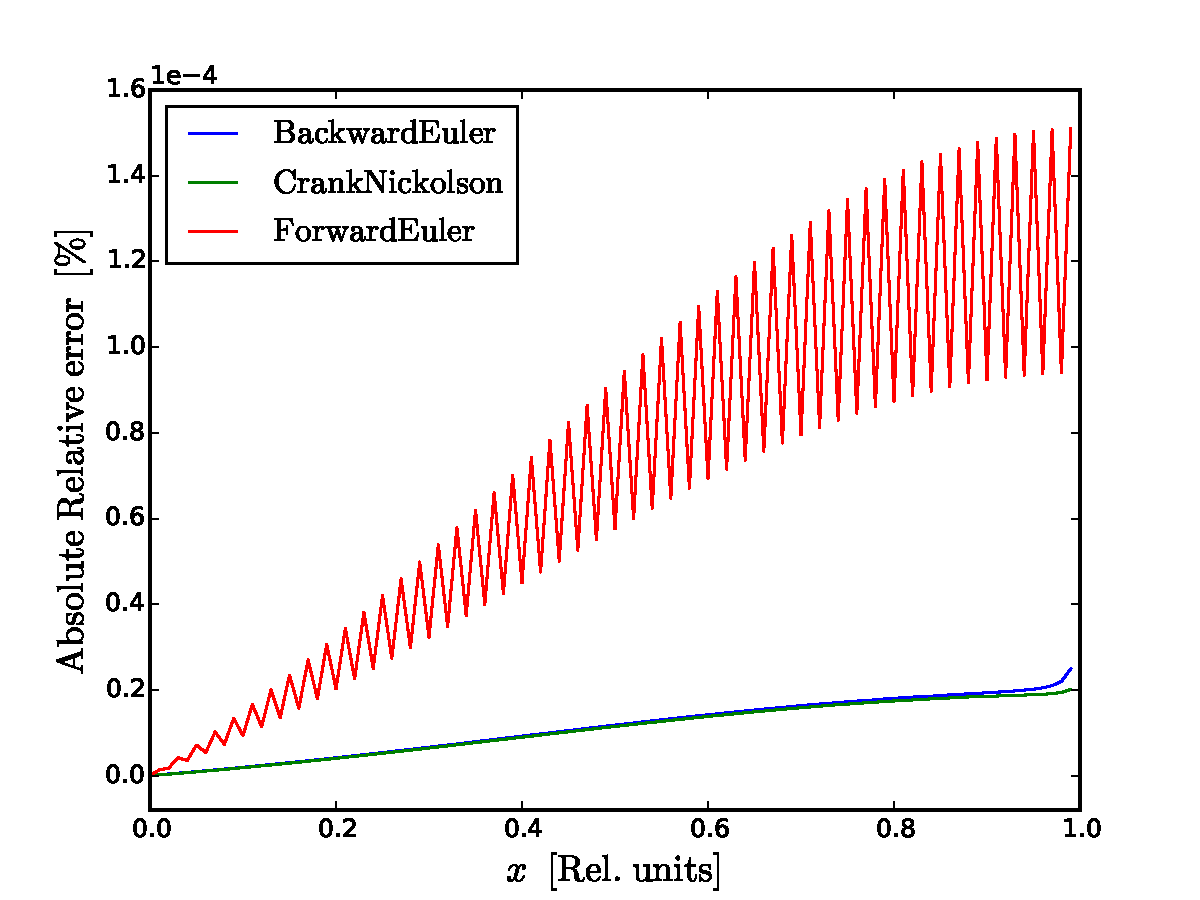
\includegraphics[width=0.49\linewidth, clip=true, trim=0 5 0 29]{Figures/FYS3150_project_5_differential_error_dx001_linear.pdf}
			
			\caption{Plot of the numerical solution of the diffusion process using the three different differential schemes using different step-length $\Delta x=1/10$ and $\Delta x = 1/100$ , at two different times in the simulation. As wee see, the solution approaches the steady state $u(x) = 1-x$.}
			\label{fig: differentials all results}
		\end{figure}}
		
	\subsection{Random walk}
		Mathematically and conceptually, the random walk methods are much simpler to implement than the above differential methods. The downside, however, is a greater demand on computation power. To achieve a good agreement with reality, one should ideally have a very large number of pending particles at the $x=0$ position, however this is not practically feasible. In my computations I have used a constant 10 000 particles at this position, but the total number of particles at the end-state showed to multiply by a factor up to and beyond 300.
		
		Fig.~\ref{fig: histogram random walkers constant step} shows the simulation when a constant step length was used, for a total time of $T=0.1$ and $T=0.3$, relative units. The figure shows quite clearly that the agreement is very quite good in both cases. 
		
		On the contrary, fig.~\ref{fig: histogram random walkers gaussian step} shows the same system, but where the walkers are moving with a normally distributed step length and the agreement is rather poor. I have here also included the plot for when I terminated the computation after a time $T=0.5$, relative units. The histogram is visibly approaching the steady state, but not at the rate the real system does, and so one can only use this method to study the steady state as $T\rightarrow \infty$.

		It is, then, obvious that the constant step length is much more desirable in problems like this one, however the very fact that the two methods produce incompatible results may provide us with important insights in the underlying physics of diffusion. 
		
		I propose, therefore, that the particles in fact \textit{are} moving with a constant step length, and that this is due to the density of the fluid through which they are moving. If the fluid is dense enough, i.e. the diffusion coefficient is large, the individual molecules in the fluid will be roughly equidistant, and so the possible spots in which the diffusive molecule can occupy (between the fluid molecules) are also roughly equidistant. Lowering the density, like for example in a gas, will influence this motion drastically and the random walkers will have a much greater chance of moving with a distributed step length. This would be an interesting topic for further research.
		
		It should also be said that the CPU-time required is much greater for the normally distributed step length, than for the constant step length, and the total number of particles after the computation is done is orders of magnitude greater in the former case.
		\begin{figure}
			\centering
			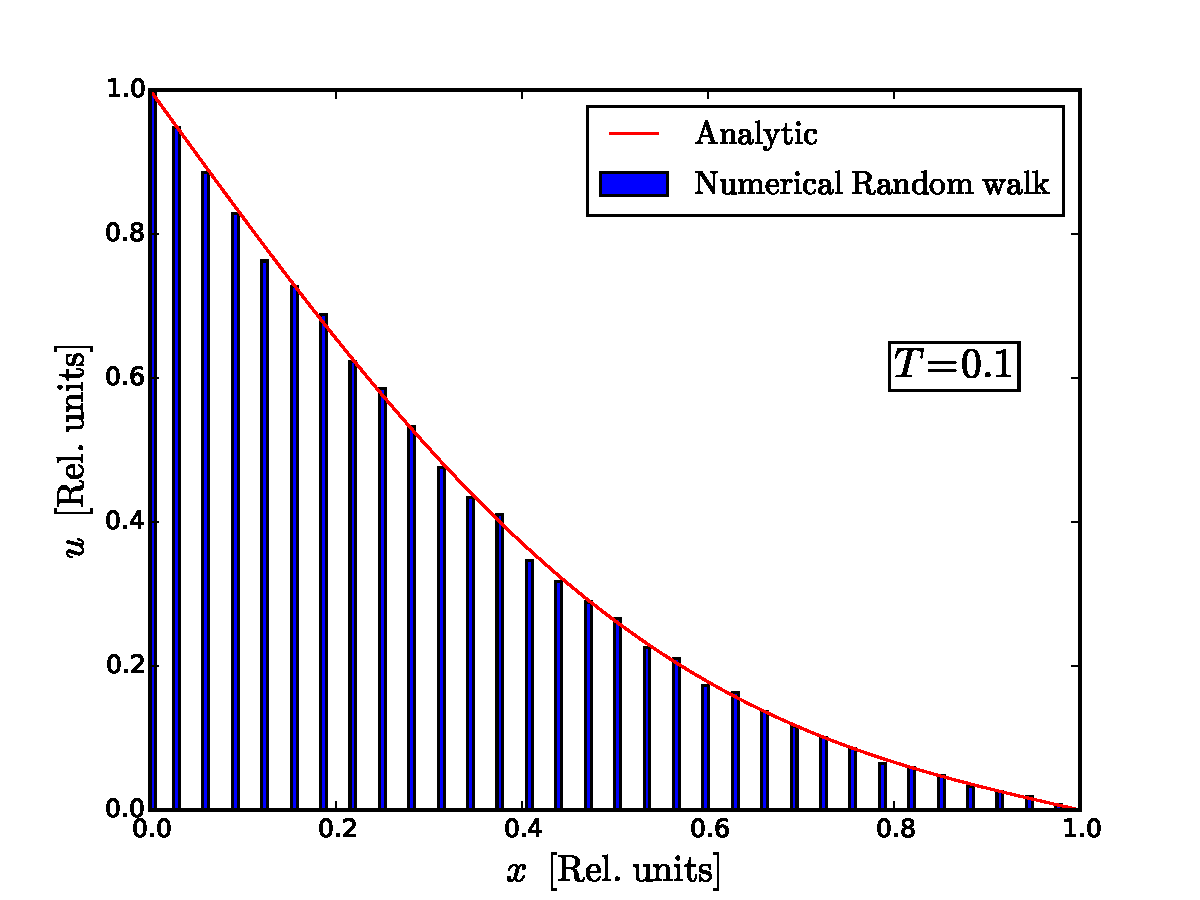
\includegraphics[width=0.5\linewidth]{Figures/RandomWalk_constant_step_T01}%
			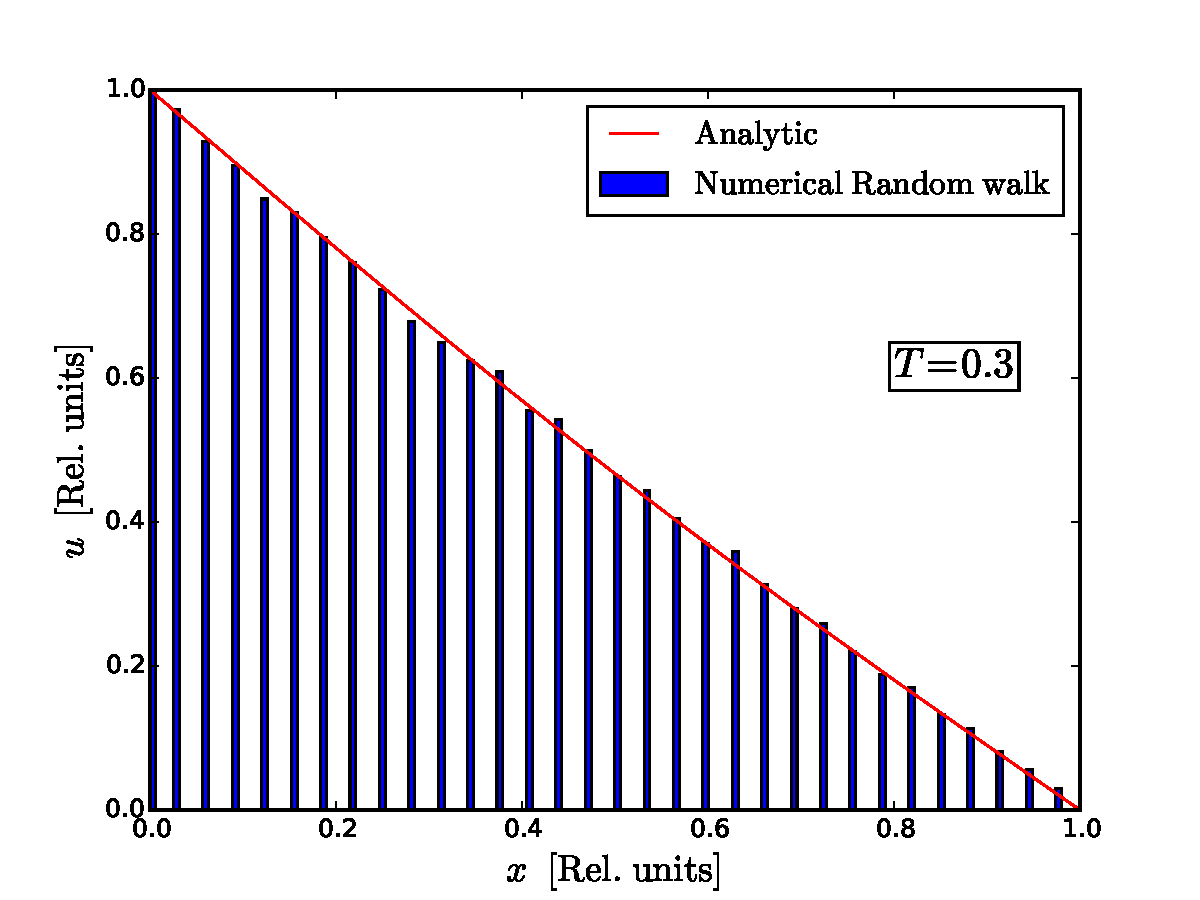
\includegraphics[width=0.5\linewidth]{Figures/RandomWalk_constant_step_T03}
			\caption{Histogram of the positions of the random walkers with constant step length. The analytical solution is also plotted, and the agreement is remarkable.}
			\label{fig: histogram random walkers constant step}
		\end{figure}
		\begin{figure}
			\centering
			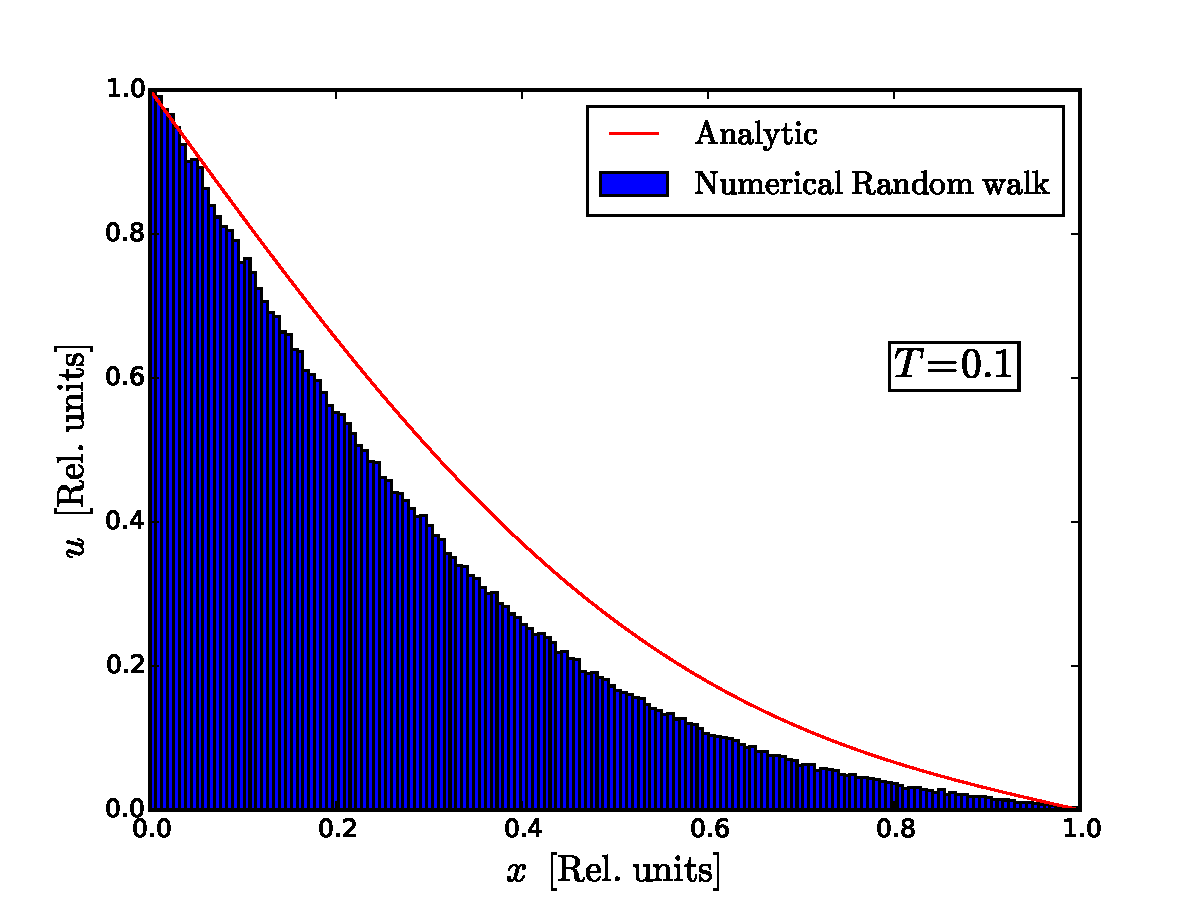
\includegraphics[width=0.5\linewidth]{Figures/RandomWalk_gaussian_step_T01}%
			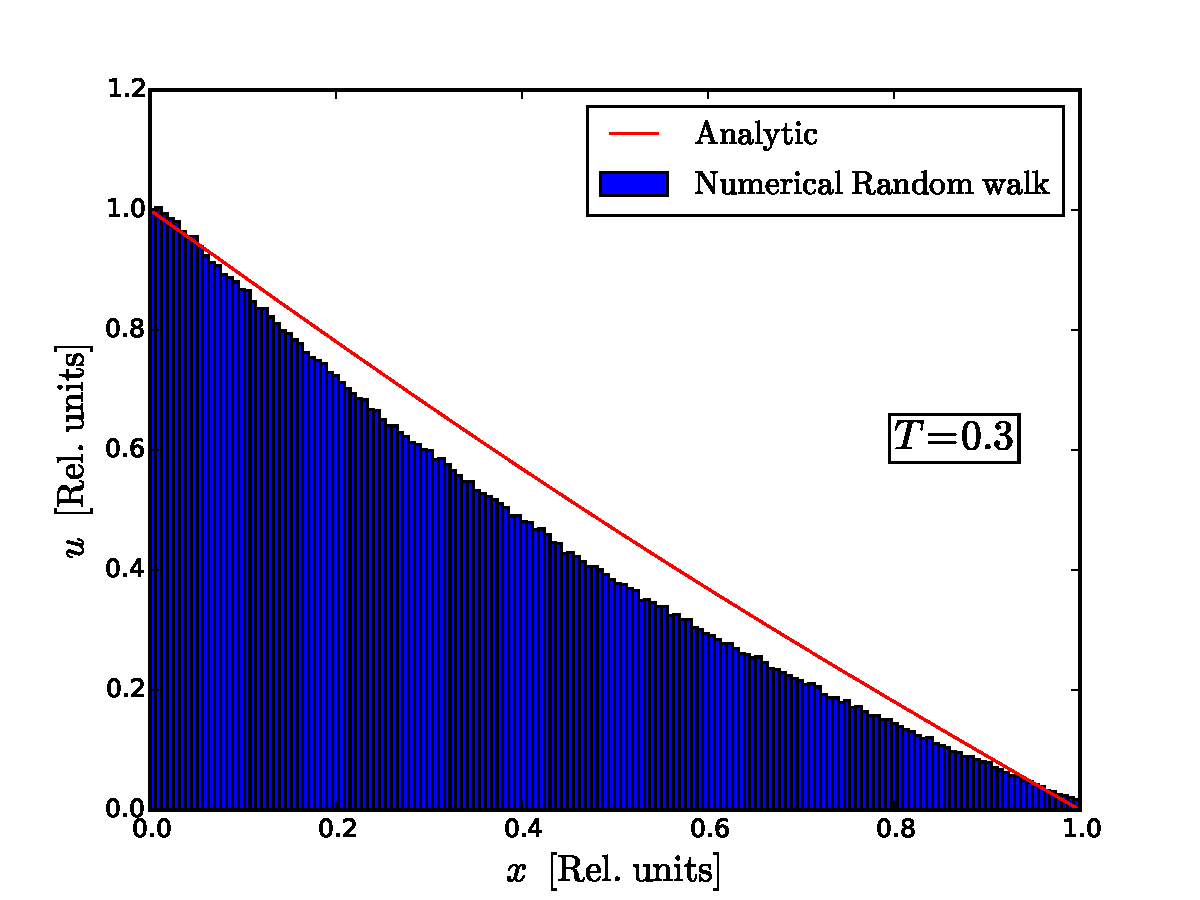
\includegraphics[width=0.5\linewidth]{Figures/RandomWalk_gaussian_step_T03}
			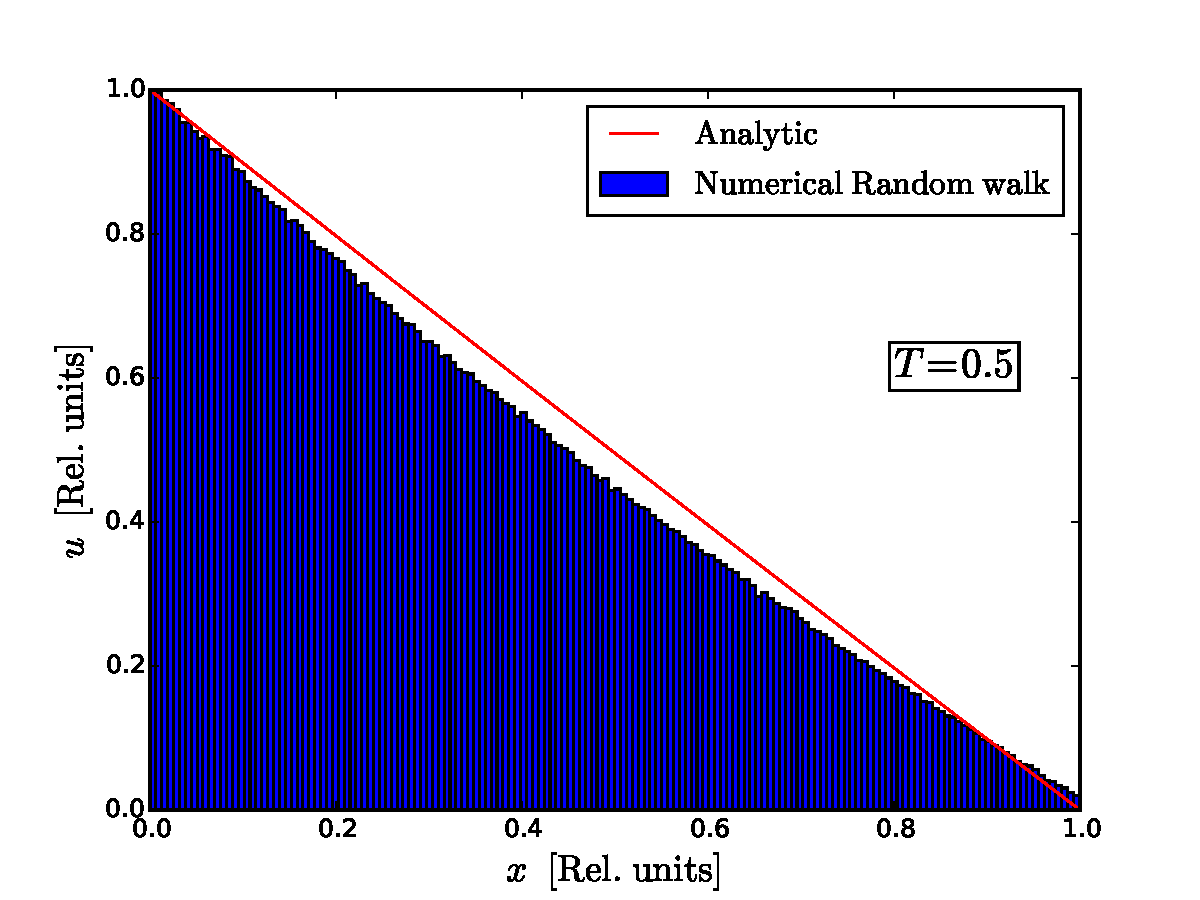
\includegraphics[width=0.5\linewidth]{Figures/RandomWalk_gaussian_step_T05}
			\caption{Histogram of the positions of the random walkers at two points in time. The walkers are moving with a random step length $l_0 = \sqrt{2\Delta t}\xi$ where $\xi$ is a random number from the normal distribution with average 0 and standard deviate 1.}
			\label{fig: histogram random walkers gaussian step}
		\end{figure}
	\subsection{Code Verification}
		I end now with a section regarding verification of the code.
		
		In the cases for differential methods, the codes have been obviously shown to work, ref fig.~\ref{fig: differentials all results}. A good test, however, is the conservation of boundary conditions, which in the cases of the backward and Crank-Nicolson schemes are hard-coded. In the case of the forward scheme, one can simply include a print statement to verify the requirement.
		
		When dealing with the random walk methods, the quantities that need to be conserved are the number of particles at $x=0$ and $x=d=1$, which should be 10 000 and 0 respectively in my calculations. The script \texttt{histplot.py} which produces the histograms in figures~\ref{fig: histogram random walkers constant step} and \ref{fig: histogram random walkers gaussian step}, also prints out these values and show that, indeed, the requirement is met.
		
\section{Conclusion}
	The 1+1D diffusion equation is possible to solve analytically, but a numerical solution provides us with a powerful tool to study any kind of diffusion processes where the physical constraints and simplifications implemented above may or may not partake. 
	
	I have shown that both the explicit (forward Euler) scheme, implicit (backward Euler) scheme and the Crank Nicolson scheme give reasonably good answers with the poorest results being only 0.4\% off the analytical answer for the explicit scheme. This falls within the margin of error of most experiments, however with a few, simple, changes the implicit or Crank-Nicolson schemes may be implemented to produce even more accurate results, the only downside being a possible limitation on the computer hardware. 
	
	I have also studied diffusion in light of a random walk process and shown that diffusion indeed is a form of random walk, but the nature of the walk is subject to further research. I have looked at a random walk process where the walkers have a constant step length and compared the results to the case where the step length was distributed. The former reproduces the analytical results beautifully, but the latter does not. I argue on the discrepancy, and propose an explanation based on the density of the diffusive medium.


\bibliographystyle{plain}
\bibliography{references}


%\end{multicols}

\end{document}
